%Dokumentenklasse "scrbook" - Erweitert um den Verweis auf die Verzeichnisse und Texteigenschaften
\documentclass[chapterprefix=true, 12pt, a4paper, oneside, parskip=half, listof=totoc, bibliography=totoc, numbers=noendperiod]{scrbook}

% Ränder (Standard bottom ca. 52mm anbzüglich von ca. 4mm für die nach oben rechts gewanderte Seitenzahl)
%Anpassung der Seitenränder
\usepackage[bottom=48mm,left=25mm,right=25mm]{geometry}

% Ränder bei Bedarf zeigen
%\usepackage{showframe}

%Tweaks für scrbook
\usepackage{scrhack}

%Blindtext
\usepackage{blindtext}

%Erlaubt unteranderem Umbrücke captions
\usepackage{caption}

%Stichwortverzeichnis
\usepackage{imakeidx}

%Kompakte Listen
\usepackage{paralist}

%Zitate besser formatieren und darstellen
\usepackage{epigraph}

%Glossar, Stichworverzeichnis
\usepackage[toc, acronym]{glossaries} % Akronyme werden als eigene Liste aufgeführt

%Anpassung von Kopf- und Fußzeile
%beinflusst die erste Seite des Kapitels
\usepackage[automark,headsepline]{scrlayer-scrpage}
\automark{chapter}
\ihead{\leftmark}
\chead{}
\ohead{\thepage}
\ifoot*{}
\cfoot[\thepage]{}
\cfoot*{}
\ofoot*{}
\pagestyle{scrheadings}

%Auskommentieren für die Verkleinerung des vertikalen Abstandes eines neuen Kapitels
%\renewcommand*{\chapterheadstartvskip}{\vspace*{.25\baselineskip}}

%Zeilenabstand 1,5
\usepackage[onehalfspacing]{setspace}

%Verbesserte Darstellung der Buchstaben zueinander
\usepackage[stretch=10]{microtype}

%Deutsche Bezeichnungen für angezeigte Namen (z.B. Innhaltsverzeichnis etc.)
\usepackage[ngerman]{babel}

%Unterstützung von Umlauten und anderen Sonderzeichen (UTF-8)
\usepackage{lmodern}
\usepackage[utf8]{luainputenc}
\usepackage[T1]{fontenc}

%Einfachere Zitate
\usepackage{epigraph}

%Verwendung von Akronymen
\usepackage[printonlyused]{acronym}

%Unterstützung der H positionierung (keine automatische Verschiebung eingefügter Elemente)
\usepackage{float} 

%Erlaubt Umbrüche innerhalb von Tabellen
\usepackage{tabularx}

%Erlaubt Seitenumbrüche mit Tabellen
\usepackage{longtable}

%Erlaubt die Darstellung von Sourcecode mit Highlighting
\usepackage{listings}

%Definierung eigener Farben bei nutzung eines selbst vergebene Namens
\usepackage[table,xcdraw]{xcolor}

%Vektorgrafiken
\usepackage{tikz}

%Grafiken (wie jpg, png, etc.)
\usepackage{graphicx}

%Grafiken von Text umlaufen lassen
\usepackage{wrapfig}

%Ermöglicht Verknüpfungen innerhalb des Dokumentes (e.g. for PDF), Links werden durch "hidelink" nicht explizit hervorgehoben
\usepackage[hidelinks,german]{hyperref}

%Einbindung und Verwaltung von Literaturverzeichnissen
\usepackage{csquotes} %wird von biber benötigt
\usepackage[style=alphabetic, backend=biber, bibencoding=ascii]{biblatex}
\addbibresource{references/references.bib}

%-------------------------------Zusätzliche Anpassungen und Modifikationen--------------------------------------------%

%Anpassung der Überschriften
\addtokomafont{disposition}{\rmfamily}

%Zusätzliche Farben
\definecolor{darkgreen}{RGB}{0,100,0}

%Umbenennungen
\renewcommand{\lstlistlistingname}{Quelltextverzeichnis}

%Pluszeichen in der Referenc beim zitieren ausblenden
\renewcommand*{\labelalphaothers}{}

%Anpassugen zur Quelltextdarstellung, kann bei Bedarf überschrieben werden (z.B. wenn unterschiedliche Sprachen zum Einsatz kommen)
\renewcommand{\lstlistingname}{Codeauszug}
\lstset{
	language=Java,
	numbers=left,
	columns=fullflexible,
	aboveskip=5pt,
	belowskip=10pt,
	basicstyle=\small\ttfamily,
	backgroundcolor=\color{black!5},
	commentstyle=\color{darkgreen},
	keywordstyle=\color{blue},
	stringstyle=\color{gray},
	showspaces=false,
	showstringspaces=false,
	showtabs=false,
	xleftmargin=16pt,
	xrightmargin=0pt,
	framesep=5pt,
	framerule=3pt,
	frame=leftline,
	rulecolor=\color{green},
	tabsize=2,
	breaklines=true,
	breakatwhitespace=true,
	prebreak={\mbox{$\hookleftarrow$}}
}

%Anpassungen für das Abkürzungsverzeichnis
\newglossarystyle{dottedlocations}{%
	\glossarystyle{list}%
	\renewcommand*{\glossaryentryfield}[5]{%
		\item[\glsentryitem{##1}\glstarget{##1}{##2}] \emph{##3}%
		\unskip\leaders\hbox to 2.9mm{\hss.}\hfill##5}%
	\renewcommand*{\glsgroupskip}{}%
}

%%Titles - Uncomment one section of titles

%%Used for titleGraduation
\makeatletter

\newcommand*{\gradeType}[1]{\gdef\@gradeType{#1}}
\newcommand*{\firstExaminer}[1]{\gdef\@firstExaminer{#1}}
\newcommand*{\secondExaminer}[1]{\gdef\@secondExaminer{#1}}
\newcommand*{\matrikelnr}[1]{\gdef\@matrikelnr{#1}}
\newcommand*{\submitDate}[1]{\gdef\@submitDate{#1}}

\renewcommand*{\maketitle}{
	\begin{titlepage}
		\newgeometry{left=2.5cm,right=2.5cm,top=9.0cm,bottom=2.5cm}
		\begin{center}
			\vfill
			{\Large \@title\par}
			\vskip 0.5cm
			{\large \bfseries Bachelor's Thesis\par}
			\vskip 0.5cm
			{\large for obtaining the academic degree\\ \bfseries \@gradeType}
			\vskip 0.5cm
			{\large at}
			\vskip 0.5cm
			{\large Beuth Hochschule für Technik Berlin\\ Department Informatics and Media VI\\ Degree Program Mediainformatics}
			\vfill
			\begin{flushleft}
				\begin{tabular}[t]{rl}
					1. Examiner and Supervisor: &\@firstExaminer\\
					2. Examiner: & \@secondExaminer\\
					\\
					Submitted by: &\@author\\
					Matriculation number: & \@matrikelnr\\
					Date of submission: & \@submitDate
				\end{tabular}
			\end{flushleft}
		\end{center}
		\restoregeometry
	\end{titlepage}
}
\makeatother
\gradeType{Bachlor of Science (B.Sc.)}
\secondExaminer{Prof. Dr. Elmar Böhler}

%%Used for titleResearchPaper
%\makeatletter

\newcommand*{\firstExaminer}[1]{\gdef\@firstExaminer{#1}}
\newcommand*{\subTitle}[1]{\gdef\@subTitle{#1}}
\newcommand*{\researchPart}[1]{\gdef\@researchPart{#1}}
\newcommand*{\matrikelnr}[1]{\gdef\@matrikelnr{#1}}
\newcommand*{\submitDate}[1]{\gdef\@submitDate{#1}}


\renewcommand*{\maketitle}{
	\begin{titlepage}
		\newgeometry{left=2.5cm,right=2.5cm,top=9.0cm,bottom=2.5cm}
		\begin{center}
			\vfill
			{\Large \@title\par}
			{\normalsize \@subTitle\par}
			\vskip 0.5cm
			{\large \bfseries Forschungsprojekt Teil \@researchPart\par}
			\vskip 0.5cm
			{\large an der}
			\vskip 0.5cm
			{\large Hochschule für Technik und Wirtschaft Berlin\\ Fachbereich Wirtschaftswissenschaften II\\ Studiengang Angewandte Informatik}
			\vfill
			\begin{flushleft}
				\begin{tabular}[t]{rl}
					Betreuer: &\@firstExaminer\\
					\\
					Eingereicht von: &\@author\\
					Matrikelnummer: & \@matrikelnr\\
					Datum der Abgabe: & \@submitDate
				\end{tabular}
			\end{flushleft}
		\end{center}
		\restoregeometry
	\end{titlepage}
}
\makeatother
%\subTitle{Ein optionaler Untertitel der Arbeit}
%\researchPart{A}

%%Used by all titles
\title{Design and Implementation of a Tool to Collect Execution- and Service-Data of Big Data Analytics Applications}
\author{Markus Lamm}
\matrikelnr{s786694}
\submitDate{06.09.2016}
\firstExaminer{Prof. Dr. Stefan Edlich}
%%End Titles

\makeindex[title=Index, options=-s indexstyle.ist, intoc]
\indexsetup{level=\chapter*,toclevel=chapter}

\makeglossaries
\loadglsentries{glossary_and_acronyms.tex}
\setacronymstyle{long-short}

\begin{document}

\pagenumbering{alph} %fix for same identifier warning, character is not show in title
\maketitle

\pagenumbering{Roman}

%\chapter*{Ackknowledgements}
\blindtext \clearpage
\chapter*{Abstract}

\blindtext \clearpage

\tableofcontents \newpage

\pagenumbering{arabic}
\chapter{Introduction}
\section{Motivation}
According to a survey in Germany, nine out of ten companies (89 percent) analyze large
volumes of data for operational decision-making processes using modern Big Data Analytics
Architectures, where 48 percent of the respondents see the greatest potential of Big Data
\cite{Bitk14}. The analysis of continuous data streams is taking up a growing importance
for companies and therefore constitutes an important factor for business success.

Collecting, storing and analyzing system and operational data of Big Data Architectures is
therefore an essential tool in order to ensure successful operation. Even though logfiles are
usefull for tracing problems in software systems, problems can be tracked and potential sources
of error can be identified much earlier by collecting and analyzing execution and service data at
runtime to describe the state of the system at a given point in time.

Due to the distributed character of Big Data Applications, where a system is composed of several
interacting components, the examination of log data is not an adequate choice to gain insight
into the entire system \cite{VanL14}.

\section{Objective}

The main goal of the thesis is the design and implementation of a software system to ingest
and  store system and operational data of Big Data Analytics Applications on the example of
the streaming frameworks Apache Flink and Apache Kafka. It should be examined which data is
available and can be collected at all, what data is relevant and how to collect from source
systems. Furhermore, the collected data must be stored in a persistence system to become
available for possible consumers like visualization applications, analytical processes or as
a data source for applications from the context of Machine Learning for example.

\section{Structure of thesis}

After a short introduction to the topics and the main goals of the present thesis in this
chapter, the Chapter 2 covers the theoretical foundations of Big Data Analytics
Applications, discusses the concept of "stream-processing" and introduces Apache Flink
and Apache Kafka as representatives of widely used stream-processing frameworks.

Chapter 3 investigates which sources for collecting data exist for Apache Flink and Kafka
and which data should be collected and stored in a persistence system regarding to its
relevance and data quality.

The requirements and the target definition of the software-system will be introduced
in Chapter 4, Chapter 5 describes the software solution by giving a detailed conceptional
overview of the software components and providing implementation details for selected items.

In chapter 6 we'll see how to setup the technical environment for the usage of the
prototype to verify the correct functionality related to the requirements defined in
Chapter 4.

The last Chapter 7 covers a conclusion and summary of the present work.

 \clearpage
\chapter{Basic Concepts}
After a short introduction to the terminology of Big Data and Big Data Analytics Applications
this chapter introduces the concept of stream processing, which is one of the main characteristics
of the streaming frameworks Apache Flink and Apache Kafka. The underlying concepts both of these systems
and their usage in context of Big Data Analytics will be explained at the end of this chapter.
TODO REST JMX

\section{Big Data}
In the past decade the amount of data being created is a subject of immense growth.
More than 30,000 gigabytes of data are generated every second, and the rate of data
creation is accelerating\cite{Marz15}. People create content like blog posts, tweets, social
network interactions, photos, servers continuously log messages, scientists create detailed
measurements, permanently.

\begin{figure}[H]
	\centering
	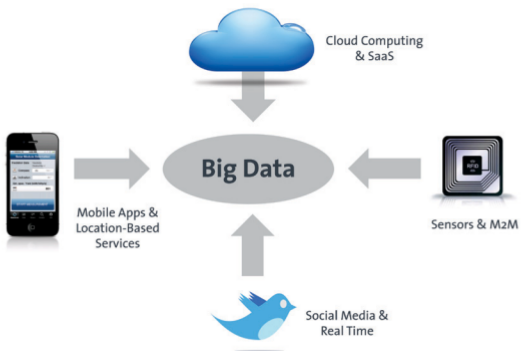
\includegraphics[width=0.55\textwidth]{../images/04-sources-of-bigdata.png}
	\caption{Sources of Big Data{\cite{Bitk12}}}
	\label{sources-of-bigdata}
\end{figure}

Through advances in communications technology, people and things are becoming in-
creasingly interconnected. Generally titled as machine-to-machine (M2M), inter-
connectivity is responsible for double-digit year over year data growth rates. Finally,
because small integrated components are now affordable, it becomes possible to add
intelligence to almost everything. As an example, a simple railway car has hundreds
of sensors for tracking the state of individual parts and GPS-based data for shipment
tracking and logistics\cite{Ziko12}.

Besides the extremely growing amount of data, the data becomes more and more diverse.
It exists in its raw and unstructured, semistructured or in rare cases in a structured form.
\cite{Bitk12} describes, that around 85 percent of the data comes in an unstructured
form, but containing valuable information what makes processing it in a traditional
relational system impractical or impossible.

According to \cite{Marz15} \cite{Ziko12}, Big Data is defined by three characteristics:
\begin{description}
    \item [Volume] The amount of present data because of growing amount of producers,
    e.g. environmental data, financial data, medical data, log data, sensor data.
    \item [Variety] Data varies in its form, it comes in different formats from different sources.
    \item [Velocity] Data needs to be evaluated and analyzed quickly, which leads to new challenges
    of analyzing large data sets in seconds range or processing of data in realtime
\end{description}
\begin{figure}[H]
	\centering
	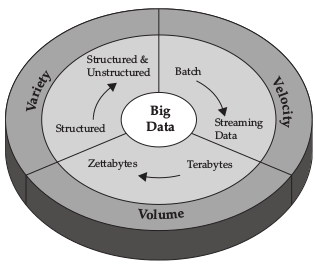
\includegraphics[width=0.5\textwidth]{../images/03-three-vs-of-bigdata.png}
	\caption{The three 'V's of Big Data{\cite{Ziko12}}}
	\label{three-vs-of-bigdata}
\end{figure}

A possible definition for Big Data could be derived as follows: \textit{Big Data refers to the use
of large amounts of data from multiple sources with a high processing speed for generating
valuable information based on the underlying data.}

Another definition comes from the the science historian George Dyson, who was cited by
Tim O'Reilly in \cite{Dys13}:
\textit{Big data is what happened when the cost of storing information became less than the
cost of making the decision to throw it away.}

According to \cite{Marz15} the term “Big Data” is a misleading name since it implies that
pre-existing data is somehow small, which is not true, or that the only challenge is the
sheer size of data, which is just one one them among others. In reality, the term Big Data
applies to information that can’t be processed or analyzed using traditional processes or
tools.

\section{Big Data Analytics Applications}
Big Data Analytics describes the process of collecting, organizing and analyzing large
volumes of data with the aim to discover patterns, relationships and other useful informa-
tion extracted from incoming data streams \cite{Marz15}. The process of analytics is typically
performed using specialized software tools and applications for predictive analytics, data
mining, text mining, forecasting and data optimization.

The analytical methods raise data quality for unstructured data on a level that allows
more quantitative and qualitative analysis. With this structure it becomes possible
to extract the data that is relevant for more detailed queries to extract the desired information.

The areas of applications may be extremely diverse and ranges from analysis of financial
flows or traffic data, processing sensor data or environmental monitoring as explained in
the previous chapter.

The illustration below summarises the six-dimensional taxonomy \cite{Bitk14, Csa14} of Big
Data Analytics Applications.
\begin{figure}[H]
	\centering
	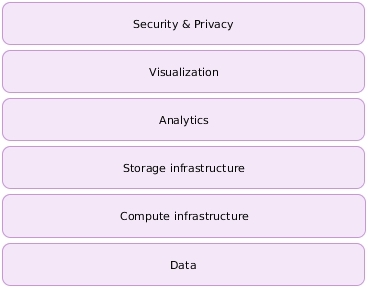
\includegraphics[width=0.5\textwidth]{../images/05-big-data-taxonomy.jpg}
	\caption{Taxonomy of Big Data Analytics Applications \cite{Bitk14, Csa14}}
	\label{taxonomy-bigdata-applications}
\end{figure}

The following section will discus the topic stream processing, which is part of the
"Compute infrastructure" layer shown in the figure above.

\section{Stream Processing}

Computing infrastructures on big data currently differ on whether the processing on streaming data
will be computed in batch mode, or in real-time/near real-time . This section is focussed on processing
continous data streams in real-time/near real-time and introduces Apache Flink and Apache Kafka as
representants of streaming frameworks.

According to \cite{Klepp16}, stream processing is the computing of data continuously,
concurrently, in real time and in a record-by-record fashion. In a stream, data isn't as treated static tables
or files, but as a continuous infinite stream of data extracted from both live and historical
sources. Various data streams could have own features, for example, a stream
from the financial market describes the whole data. In the same time, a stream for sensors
depends on sampling (e.g. get new data every 5 minutes).

The general approach is to have a small component that processes each of the events
separately. In order to speed up the processing, the stream may be subdivided, and the
computation distributed across clusters. Stream processing frameworks like Apache Flink and
Apache Kafka primarily addresses parallelization of the computational load, an additional storage
layer is needed to store the results in order to be able to query them.

This continous processing of data streams leads to the benefits of stream processing frameworks:

\begin{itemize}
	\item Accessibility: live data can be used while the data flow is still in motion and before the data being stored.
	\item Completeness: historical data can be streamed and integrated with live data for more context.
	\item High throughput: large volumes of data can be processed in high-velocity with minimal latency.
\end{itemize}

To introduce a more formal expression, a data stream is described as an ordered pair (S, T) where:
\begin{itemize}
	\item S is a sequence of tuples.
	\item T is a sequence of positive real time intervals.
\end{itemize}

It defines a data stream as a sequence of data objects, where the sequence in a data stream
is potentially unbounded, which means that data streams may be continuously generated
at any rate \cite{Nam15} and leads to the following characteristics:
\begin{itemize}
	\item the data arives continous
	\item the arrival of data is disordered
	\item the size of the stream is potentially unbounded
\end{itemize}

After this short introduction to the basics of stream processing, the following sections
covers a short introduction of the streaming frameworks Apache Flink and Apache Kafka.
\subsection{Apache Flink}

As described in the documentation \cite{Flink16}, \textit{"Apache Flink is an open source platform for
distributed stream and batch data processing. Flink’s core is a streaming dataflow engine that
provides data distribution, communication, and fault tolerance for distributed computations over
data streams. Flink also builds batch processing on top of the streaming engine, overlaying native
iteration support, managed memory, and program optimization."}

The main components of Flink applications are formed by streams and transformations, in which
streams define intermediate results whereas transformations represent operations computed on one
or more input streams with one or more resulting streams.

To illustrate the main components of a Flink application, the following code from \cite{Flink16} shows
a working example of a streaming application, that counts the words coming from a web socket in 5
second windows:

\begin{lstlisting}[caption={Basic Apache Flink streaming application}, captionpos=b, label={lst:basicflink}]
public static void main(String[] args) throws Exception {
        StreamExecutionEnvironment env = StreamExecutionEnvironment.getExecutionEnvironment();
        DataStream<Tuple2<String, Integer>> dataStream = env
                .socketTextStream("localhost", 9999)        *(1)
                .flatMap(new Splitter())                    *(2)
                .keyBy(0)                                   *(2)
                .timeWindow(Time.seconds(5))                *(2)
                .sum(1);                                    *(2)

        dataStream.print();                                 *(3)
        env.execute("Window WordCount");
    }

    public static class Splitter implements FlatMapFunction<String, Tuple2<String, Integer>> {
        @Override
        public void flatMap(String sentence, Collector<Tuple2<String, Integer>> out) throws Exception {
            for (String word: sentence.split(" ")) {
                out.collect(new Tuple2<String, Integer>(word, 1));
            }
        }
    }
\end{lstlisting}

On execution, Flink applications are mapped to streaming dataflows, consisting of streams
and transformation operators (3) where each dataflow starts with one or more sources (1)
the data is received from and the resulting stream will be written in one or more sinks (3).
to.

The dataflows of Apache Flink are in inherently parallel and distributed, by splitting streams into
stream partitions and operators into operator subtasks, which are execute independently from each
other, in different threads and on different machines or containers.

For the distributed processing of dataflows, Flink defines two type of processes:

\begin{enumerate}
    \item JobManagers (master process). At least one is required, it coordinates the
    distributed execution and is responsible for scheduling tasks, coordinate recovery
    on failures, etc.
    \item TaskManagers (worker processes) At least one is required, it executes the tasks, more
    specifically, the subtasks of a dataflow, and buffer and exchange the data streams.
\end{enumerate}

A basic Flink cluster set up with a single JobManager and TaskManager on Docker will be introduced in
Chapter 5 Evaluation and serves as source to collect data from, as well as a streaming component for
processing collected data.

In addition, Apache Flink provides a client, which is not part of the runtime. It is used as a part
of Java/Scala applications to create and send dataflows to the JobManager. The client will
be used in the software component "CollectorDataProcessor" and introduced in Chapter 4 Architecture
and Implementation.

\subsection{Apache Kafka}

Apache Kafka is publish-subscribe queuing service rethought as a distributed commit log \cite{Kafka16},
supporting stream processing with millions of messages per second, durability of messages through disk
storage and replication accross multiple machines in clustered environments. It is written in Scala, was
initially developed at LinkedIn and follows the distributed character of Big Data Analytics Applications
by it's inherent design.

This excerpt from the paper \cite{Neha11} the team at LinkedIn published about Kafka describes the
basic principles:

\textit{A stream of messages of a particular type is defined by a topic. A producer can publish
messages to a topic. The published messages are then stored at a set of servers called brokers.
A consumer can subscribe to one or more topics from the brokers, and consume the subscribed
messages by pulling data from the brokers. (…) To subscribe to a topic, a consumer first creates
one or more message streams for the topic. The messages published to that topic will be evenly
distributed into these sub-streams. (…)  Unlike traditional iterators, the message stream iterator
never terminates. If there are currently no more messages to consume, the iterator blocks until
new messages are published to the topic.}

A common use case for Apache Kafka in the context of stream processing is the buffering of messages
between stream producing systems by providing a queue for incoming and outgoing data. According
to the explanation of the concept of data sources and sinks in the Apache Flink section above, Apache Kafka
is heavily used as an input source, as well as output sink for the processing dataflow in Apache Flink
applications.

The following figure shows a typical use case for a data pipeline that typically start by pushing data
streams into Kafka, consumed by Flink applications, which range from simple data transformations
to complex data aggregations in a given time window. The resulting streams are written back to Kafka
for the consumption by other services or the storage in a persitent medium.
\begin{figure}[H]
	\centering
	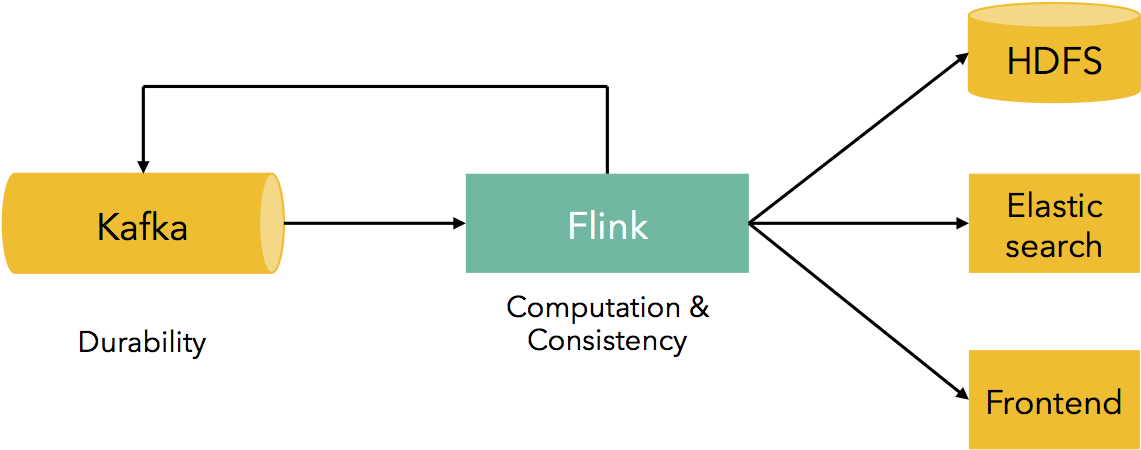
\includegraphics[width=0.7\textwidth]{../images/05-kafka-flink-pipeline.png}
	\caption{A typical Kafka-Flink pipeline{\cite{Dartisans15}}}
	\label{kafka-flink-pipeline}
\end{figure}

Chapter 5 Evaluation describes the Docker setup for a single Kafka node that is part of the
software solution in addition of provisioning data for collection.

\section{Representational State Transfer (REST)}
In his doctoral dissertation from 2000 titled "Architectural Styles and the Design of Network-based
Software Architectures", Roy Thomas Fiedling introduced the term Representational
State Transfer (REST) as core set of principles, properties, and constraints defining an "architectural
style for distributed hypermedia systems"\cite{Field00}. To understand the way of data exchange of the software system
coming in Chapter 5 Architecture and Implementation, an excerpt of relevant characteristics of REST architectures will be
discussed in this section.

REST architectures must meet the following characteristics, et al:
\begin{enumerate}
    \item \textbf{Client-Server architecture:}
    Clients and servers are separated by a uniform interface to facilitate portability. For example, a user interface
    is not concerned with data storage because it is internal to the server. On the other hand, the server is not concerned
    with the user interface or state. As long as the interface is not altered, the separation of concerns enables the
    components to evolve independently and thereby the improves scalability of the entire system.
    \item \textbf{Stateless:}
    The communication between clients and server must be stateless. Each request from any client contains all the
    information necessary to service the request, and session state is held in the client.
    \item \textbf{Uniform Interface:}
    The uniform interface between the interacting components is a fundamental characteristic of REST architectures and subjects
    to the following constraints:
    \begin{enumerate}
        \item \textbf{Identification of Resources:}
        Resources describe any information that is originated on the server and can be be identified using URIs in web-based
        REST systems. The resources themselves are conceptually separate from the representations that are returned to the client.
        For example, the server may send data from its database as JSON data or HTML web page, what is diffent to the server's
        internal representation.
        \item \textbf{Manipulation of Resources through Representations:}
        The modification of the resource is performed by using the representation. If the representation and attached metadata
        is available, clients are able to change the state of the resource by modifying or deleting the resource.
    \end{enumerate}
\end{enumerate}

Chapter 4 Architecture and Implementation will apply these principles to enable the exchange of data between distributed
software components by using an uniform interface based on the on Hypertext Transfer Protocol and the the corresponding HTTP
verbs (GET, POST, PUT, DELETE,..).

\section{{Java Management Extensions (JMX)}}

General JMX explanation, data access MBeansServerConnection

\section{Summary}

TODO \clearpage
\chapter{Requirements Analysis and Specification}

After a short introduction to the basic concepts of Big Data, Big Data Analytics Applications
and Apache Flink and Apache Kafka as examples for streaming frameworks, this chapter
examines what different kind of data are available  for both of the systems and should be
transported to a central storage system. According to the results of the data analysis, the
functional and non-functional requirements of the software system which is forming the core of
the present thesis will be defined.

\section{Data Analysis}

live and historical sources

"COLLECT EVERYTHING!

%What to Transport? Logs vs. Metrics see http://blog.mmlac.com/log-transport-with-apache-kafka/
%The first consideration should be if it is possible and/or necessary to transport all logs to a central location. If there are many servers or a lot of log data, this might be very resource intensive and aggregating or filtering the data might be necessary. The extremes of this are either transporting every single log vs. only transporting aggregated metrics. The following paragraphs try to help you decide on the right balance for your use case.
%
%Advantages of transporting all logs:
%
%Metrics can be added, modified and deleted in one central location
%Historical data on new metrics can be computed from the stored logs
%Possibility to peek into live data-stream
%Allows building complex debugging and monitoring tools
%Central location for all logs. Invaluable for debugging, root-cause analysis and correlation of incidents
%Advantages of transporting only metrics:
%
%Transporting (aggregated) metrics requires far less bandwidth
%Smaller storage requirements
%Scales far better
%Better than nothing
%Overall transporting all logs has many advantages and should be preferred over aggregated metrics if possible. Especially managing metric definitions in one place and the ability to compute historic data for new metrics is very valuable. Also does transporting all logs allow for thorough (computationally expensive) data analysis on historic data to i.e. train machine learning models, predict behavior or give enhanced insights into who your users are and what they do.
%
%There is no strict rule to follow and it is perfectly ok to mix and match. An example would be to just transport logs that contain examinable data and aggregate performance metrics, like average response time or jobs processed per minute, on the server.
%
%This post will focus on the transport of raw log data. The posts “Server Monitoring with Sensu” and “Metrics with Graphite” will introduce better suited technologies to work with pure metrics.

\subsection{System data}

Observation of cpu-, disk- and memory-utilization, why.
Dstat system util introduction

\subsection{Application data}

Apache Flink provides application data via Monitoring REST API, describe REST
Since version 1.1.0 new Metrics data via JMX
Analyze Flinks REST data

\section{Data Quality}

Define DQ, evaluate quality for data above

\section{Functional Requirements}

Describe "big picture" functionality see \cite{VanL14}, follows distributed character of Big Data Analytics
Applications, provide "on demand" data collection, as much data as possible, realtime?, three main components,
break down for:

\subsection{Collection}

collect data in clustered environments

\subsection{Transport}

Scalability with message broker

\subsection{Persistence}

Accessibility for AI, UI applications

\section{Non-Functional Requirements}

Performance, scalability,
%simplicity, modifiability, visibility, portability, and reliability

\section{Summary} \clearpage
\chapter{System Architecture}
\label{ch:architecture}

%Welche Teilprobleme leiten sich aus der Zielstellung weiter ab?
%Was sind die Rahmenbedingungen für die Probleme und wie können wir diese lösen.
%Wie können wir die Probleme formalisieren? Und daraus schlussfolgern, ob sich
%existierende Lösungen ableiten lassen.
%Methodik/Vorgehen (diesmal ausführlich)
%●
%Bauen Sie auf der Methodik aus der Einführung auf.
%Ein System bauen und dann beobachten (machen Sie wohl meistens)
%Analytisch (sie prüfen ein mathematisches Gerüst/Algorithmus/ Theorem)
%Jemanden aktiv Fragen (wahrscheinlich eher in den meisten Fällen nicht)
%Übersicht bzw. Architektur
%●
%z.B. wenn Sie ein System bauen. Wie sieht Ihre Architektur aus? Was sind die Resultate des
%Entwurfs? Welche Alternativen gibt es zu Ihrem Entwurf? Warum haben Sie sich gerade für
%Ihre Lösung entschieden? Was sind deren Vor­ und Nachteile?
%Welche Prozesse unterstützt die Architektur?
%Datenquellen?
%Transformationen?
%Datenverarbeitung? ●
%Anfrage­Schnittstellen
%Oder aber: Der xxx Algorithmus
%●
%Eigenschaften des Algorithmus, Komplexität
%Wie gehen Sie vor?
%Beschreiben Sie was wann passiert
%Optional: Der yyyy Algorithmus
%●
%Eigenschaften des Algorithmus, Komplexität
%Wie gehen Sie vor?
%Beschreiben Sie was wann passiert
%Zusammenfassung (ca. 0,5 Seiten)
%●
%Was haben wir in diesem Kapitel gelernt?
%Wie passt das zur Zielstellung der Arbeit
%Wie passt das zum nächsten Kapitel?

After the context in which the solution is settled has been described in \autoref{ch:basic-concepts}, \autoref{ch:requirements}
inspected Apache Flink and Apache Kafka according available sources of data and evaluated the data based on the quality. As
a result, the functional and non-functional requirements had been defined. According to the main goals of this thesis,
the collection of system and application data from Apache Flink and Apache Kafka and storage of collected data in a
centralized persistence system, the following sub-problems had been identified:

\begin{enumerate}
    \item Both source systems operate as distributed systems which consists of multiple instances of Apache
    Flink Job- and TaskManagers or Apache Kafka brokers, producers and consumers respectively. The software solution proposed
    must enable the collection of data from multiple application instances to gain an overall picture of the entire system.
    \item The process of data collection mustn't cause a negative impact on source systems. Since Apache Flink and Apache Kafka
    are both systems processing large amounts of data very fast, the utilization of system resources like cpu and memory of the
    collecting system must be kept as low as possible.
    \item As a result, the data must be transfered to the storage system with as less input/output operations and as fast
    as possible, to become available for possible data consumers immediately.
    \item The system architecture must provide a mechanism for the integration of possible data consumers which are unknown at
    the point of this thesis.
\end{enumerate}

The following chapter introduces the \textit{"Collector-Platform"} as a pipeline of data collection, transport and storage with the purpose
to collect data of distributed Apache Flink and Kafka systems and make it available for consumers that are potentially unknown at present
as fast as possible. The components will be discussed at architectural level, whereas implementation details follow in \autoref{ch:implementation}.

\section{The "Collector-Platform"}

According to the requirements in \autoref{ch:requirements}, the \textit{"Collector-Platform"} is responsible to perform the
following operations, which describe the pipeline the data in running throught on each source system. Irrespective of the source system,
the sequence remains the same for Apache Flink and Kafka or any other source system observed, it just differs in the implementation of
data collection processes:

\begin{figure}[H]
	\centering
	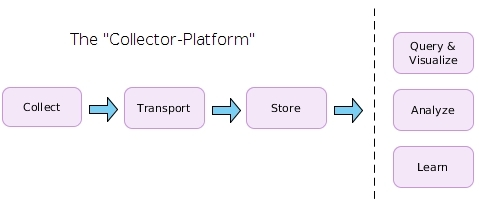
\includegraphics[width=0.8\textwidth]{../images/06-collect-pipeline.jpg}
	\caption{Collector Pipeline, \cite{VanL14}}
	\label{fig:colletor-pipeline}
\end{figure}

The the first step is the collection of data defined in \autoref{ch:requirements} on the Apache Flink and Apache Kafka source
systems. This includes collection of system data with the Dstat system utility as well as application specific data provided
by JMX or REST respectively. Once the the corresponding data had been retrieved and converted into a structured JSON format,
the data must leave source systems in the second step to reach the storage system at last, where they become available for
visualization tools, analytical processing or as a source for Machine Learning applications. \autoref{ch:evaluation} introduces
a sample application to demonstrate the possibilities for the integration of data consumers using the Stream Processing capabilities
of Apache Flink.

The "Collector-Platform" consist of the following components and will be discussed in the corresponding sections:

\begin{itemize}
    \item CollectorClient
    \item CollectorManager
    \item Consul ClientRegistry
    \item Kafka Message-Broker
    \item Logstash-Processor
    \item Elasticsearch Index
\end{itemize}

The following diagram shows an overview of all components involved and the interactions between them to fulfil the
requirements of data collection, transport and storage on the example of one Apache Flink JobManager and TaskManager as
source systems.

\begin{figure}[H]
	\centering
	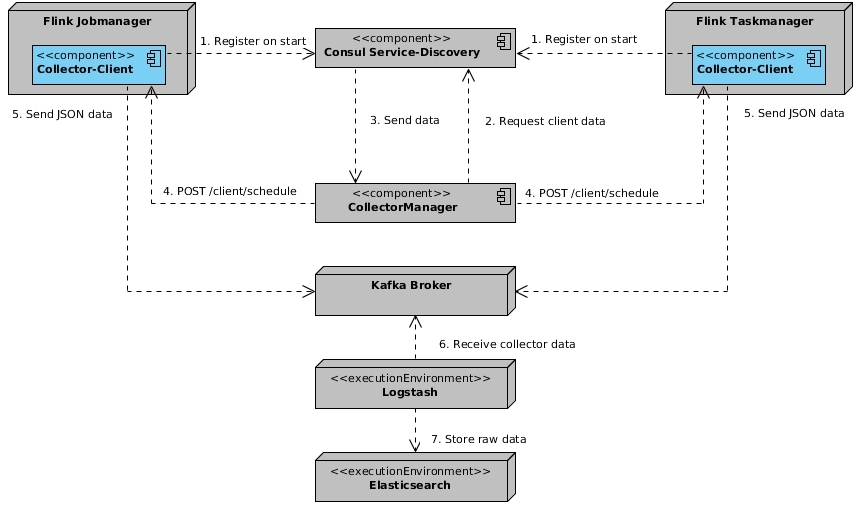
\includegraphics[width=1.0\textwidth]{../uml/component-diagram.jpg}
	\caption{The "Collector-Platform"}
	\label{fig:collector-platform}
\end{figure}

The \textit{CollectorClient}s installed on source systems, registers itself on application start with a central client registry, using
an unique identifier \verb|collector-client| \textbf{(1)}. This registry manages all registred clients and provides an interface
that allows the \textit{CollectorManager} to fetch network location (IP address and port) data for all clients that is required
to address the individual clients. The \textit{CollectorManager} uses this interface to display a list of all registred
\textit{CollectorClients} in a basic HTML user interface \textbf{(2,3)}. In addition, \textit{CollectorManager} fetches additional
meta information of the client \textbf{(4)}, like its host name and registered \textit{Collector}s, provided by the implementation
of the \textit{CollectorClient}.

In the next step, the process of data collection can be triggered using the \textit{CollectorManager}s user interface \textbf{(5)}.
Therefore, the \textit{CollectorManager} sends a HTTP \verb|POST| request with an appropriate JSON request body and receives a
status response that containing the status of the \textit{CollectorClient} that can be \verb|RUNNING| or \verb|STOPPED|,
according to the action that is triggered by the web user interface.

Now, the \textit{CollectorClient} is active and collects data corresponding the \textit{Collector} implementations registered in
the clients internal registry, see \autoref{sec:impl-collector-client}. Once all data of a single
\textit{Collector} implementation has been collected and transformed into a structured JSON format, the result will be enriched
with a client timestamp and the clients identification given by the IP address and the port the client is availabe at, and published to the
\textit{Kafka Message-Broker} \textbf{(6)}.

The \textit{Kafka Message-Broker} is the next step in the data pipeline and is the integration point for possible consumers
of data received by distributed \textit{CollectorClient}s. Due to the publish-subscribe principle Apache Kafka is based on,
potential consumers just need to subscribe to the \verb|collector-outbound-topic| for the data to become accessible.

The Logstash-Processor is the primary consumer of the data produced by \textit{CollectorClient}s. It receives outgoing \textit{CollectorClient}
data by subscribing to the \verb|collector-outbound-topic| topic, the clients publish the data into \textbf{(7)}. The Logstash-Processor performs
two essential tasks: it creates the required indexes for storing the data in Elasticserach and converts incoming data into an internal
message format that allows the data to be stored in Elasticsearch.

The Elasticsearch Index ist the last step in the \textit{"Collector-Platform"} \textbf{(8)}. It is the data sink where all collected data will be stored at.
The data is now available for querying or visualization.

For a deeper understanding, the following sections introduce the components and their corresponding functions described above.
Chosen frameworks and technologies will not be discussed in much detail, but it will be explained why each technology or
approach has been chosen.

\section{The "Collector" implementations}

This set of classes builds the core for collecting data on source systems and takes the responsibility for fetching
system data (\autoref{tbl:dstatcategories}) with the Dstat system tool as well as application data for Apache Flink
and Apache Kafka using the JMX interface (\autoref{tbl:jmxjvmdata}) and via REST for Apache Flink only
(\autoref{tbl:http-api-flink}). As shown in \autoref{ch:implementation}, all implementations are based on the
\textit{Collector} interface, what enables the handling of different realizations of data collection in a uniform way.

\section{CollectorClient}

The CollectorClient is main entry point for bringing data into the platform and belongs to the "Data" layer according to
\autoref{img:taxonomy-bigdata-applications}. It is a simple Java application and will have to be installed on source systems.
The module uses the concrete \textit{Collector} implementations described above, according to the source system and
depending on which \textit{Collector}s are registered in the client. The client contains and internal registration to enable
a mechanism to add or remove \verb|Collector| implementations without the need to change the implementation of the
\textit{CollectorClient}.

For the scheduling purposes of the collection process, the client provides a REST resource that enables the start and stop of data
collection from the HTML user interface provided by the \textit{CollectorManager} component.
This endpoint is available under the location \verb|http://{client-host}:{client-port}/client/schedule| and expects HTTP \verb|POST| requests
with a request body containing JSON data with an appropriate \textit{ScheduleRequest} for starting/stopping the data collection process.

Once started, the collection process that will be triggered by the client itself in a configurable interval, which is 5 seconds by default,
the resulted data will be send to an Apache Kafka topic called \verb|collector-outbound-topic|. The name of the topic explains the
purpose of the topic, it acts as the data sink for \textit{CollectorClient}s and separates the clients as the producing compontent
from data consumers.

Besides the scheduling REST resource, the client contains an endpoint \newline \verb|http://{client-host}:{client-port}/client/metadata|
that provides metatdata for the individual client and is required for displaying more detailed information about the client in the
\textit{CollectorManager}.

Accourding on the \verb|Collector| implementations registered in an internal registry, the client creates a continous stream
of \verb|Collector| data, a stream of "immutable facts" concerning the the system and application state of the underlying source
system at a given point of time. Every data event created by the client contains the client's timestamp, the IP address and the port thus the
origin of the data can identified. Appendix A contains the full JSON results for all available \textit{Collector} implementations.

The client follows the approach to operate in a process that is separated to the JVM process the source system is running in.
To enable the \textit{CollectorClient}s to access to the management interfaces introduced in \autoref{tbl:jmxjvmdata} on the remote JVM
of Apache Flink and Apache Kafka, the source system must to be configured to allow the connection from a remote JMX client. \autoref{ch:evaluation}
explains the adjustments that had been made on the example of Apache Flink. This in turn brings the disadvantage of potential
security risks that occur by allowing remote connections on a given port.

An alternative would have been to use the capabilities of dynamic bytecode intrumentation provided by the core of Java. Because
Apache Flink and Apache Kafka both are based on the JVM, it would have been possible to instrument the Flink or Kafka process itself,
to perform the data collection in the same process. This approach was not pursued in this thesis, because the instrumentation causes
a performance impact, that can be avoided by separation of collection in an individual process.

\section{CollectorManager}
\label{sec:arch-collector-manager}
Due to the fact that Apache Flink and Apache Kafka are composed of several interacting components and thus building
a distributed system, the \textit{"Collector-Platform"} itself builds a distributed system. Based on the requirement to provide a
mechanism to schedule the collection process in distributed \textit{CollectorClient}s, the \textit{CollectorManager} represents the management
component for the distributed system of clients by providing an overview of registered clients in the platform and
the possibility to start/stop individual clients using an HTML based user interface.

\begin{figure}[H]
 	\centering
 	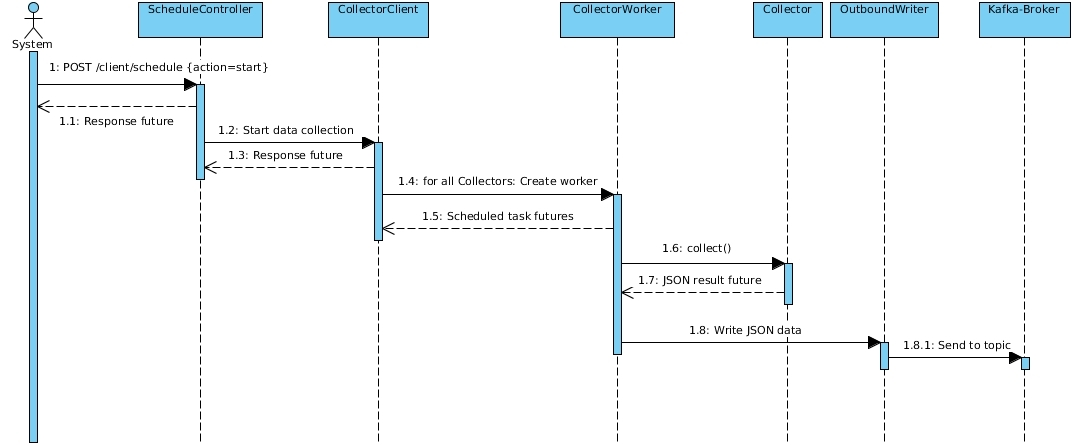
\includegraphics[width=1.0\textwidth]{../uml/sequence-scheduling.jpg}
 	\caption{Sequence diagram 'Client scheduling'}
 	\label{fig:sequence-client-scheduling}
 \end{figure}

The sequence diagram above presents the process of starting an individual \textit{CollectorClient}. The client receives a HTTP
\verb|POST| request that contains an appropriate \textit{ScheduleRequest} for starting the client. If the request is syntactically
correct, the client starts data collection as discussed above.

\section{Consul Client-Registry}

The \textit{Client-Registry} is a dedicated web service and acts as a central registry for all data collecting components
in the platform and makes the information about registered \textit{CollectorClient}s available for the \textit{CollectorManager} instances.
For the realization of an public registry for distributed clients, the platform uses Consul, a service-registry, that enables the discovery
of web services based on unique identifiers instead of host address and port information. Since the \textit{CollectorClient} is a web service itself,
clients register itself under the service name \verb|collector-client| when the client application is started. The \textit{CollectorManager}
queries the Consul node for existing instances of services named \verb|collector-client| which results in a list of registred client instances,
that contains the required information like host and port for using the scheduling and metadata endpoints in the managers user interface.

\begin{figure}[H]
	\centering
	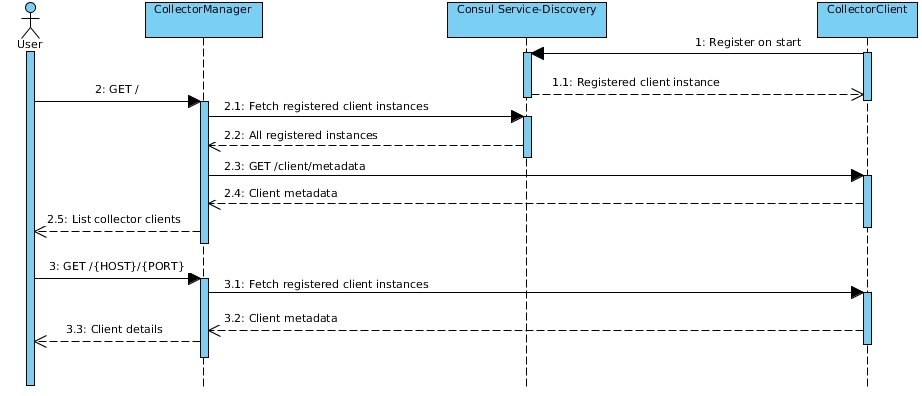
\includegraphics[width=1.0\textwidth]{../uml/sequence-discovery.jpg}
	\caption{Sequence diagram 'Client discovery'}
	\label{fig:sequence-client-discovery}
\end{figure}

Using an central registry instance for discovering \textit{CollectorClient} instances decouples the \textit{CollectorManager} from the
need to know detailed client information required for the localization of the service. Due to the fact that
client addresses and ports are dynamically assigned and may change in distributed cloud environments, the service registry provides
a scalable and flexible way to discover the providers of a given service name.

\section{Kafka Message-Broker}

The Apache Kafka Message-Broker integrates distributed \textit{CollectorClient}s to an overall system by providing a
message queue for transporting data from clients to the Logstash-Processor. The CollectorClients can publish
its data to the queue and the other applications can asynchronously read it from the queue at any time.
The usage of Apache Kafka as a publish-subscribe queuing service allows a separation of \textit{CollectorClient}s as publishers and the
Logstash-Processor and other potential as subcribers by buffering messages between stream producing systems.

\section{Logstash-Processor}
%

TODO
Receive messages from Message-Broker, route data, create ES index, why, describe context BDAA, compute layer
%
\section{Elasticsearch Index}
TODO
ES as search index for time-series based data, easy visualization with Kibana, why?, searchable, common in BDA, storage layer

\section{Summary}

open jmx port
Summarize architecture, discuss benefits and disadvantages.

%software solution is a streaming platform itself

%READ
%Messaging is the art of moving message across the producer and consumer
%group. It integrates distributed applications to an overall system by providing
%message queues for communication between them. One application can publish
%its messages to the queue and the other application can asynchronously read it
%from the queue at any time. Message Broker systems persist incoming
%messages in an enhanced type of a message queue, named topic. Sending
%messages to the broker in the form of publishing to a specific topic and on the
%other hand receiving messages only for the specified topic, is called publish /
%subscribe and this therefore classifies Kafka as a publish subscribe system.

%3.3 What is a Topic in Kafka?
%Kafka provides a high-level abstraction called Topic. Users define a new Topic
%(file) for each new category of messages (documents) and the messages are
%published to a category or stream name. A topic allows the message broker to
%deliver messages to multiple independent consumers.
%Kafka has a very simple storage layout. Each partition of a topic (file)
%corresponds to a logical log. Each time a producer publishes a message to a
%topic, the broker appends the message to the last segment file. The message is
%exposed to the consumers after it is flushed.
%
%3.4 Who are Producers in Kafka?
%Producers are the clients publishing messages to a Topic. Producers are diverse
%in nature and publish varied messages to different topics. A producer can
%publish data to a topic of its choice and is responsible for choosing which
%message will be assigned to which partition within a topic. Kafka producer client
%is configured to send messages in either a synchronous or asynchronous
%fashion to the topics. The asynchronous mode allows the client to batch small
%messages into larger data chunks before sending them over the network.
%
%3.5 What is a Message Broker?
%A Message Broker is a key element of the solution. It is a dedicated component
%which decouples the source and target systems by assuming full responsibility
%for coordinating communication between all the connected nodes. The
%published messages are stored at a set of servers called Brokers. Each Kafka
%cluster consists of one or more Brokers. The partitions of a Topic are distributed
%over the Brokers of the Kafka cluster with each Broker handling data and
%requests for a share of the partitions. Each partition is replicated across a
%configurable number of Brokers for fault tolerance. The main tasks of a message
%broker are the dynamic registration of endpoints, determining the location of a
%target system, and performing the communication as well as the transformation
%of a message from one format to another.
%A consumer can subscribe to one or more topics from the brokers and consume
%the subscribed messages by pulling data from the Brokers. The Broker locates
%the requested message by searching the list and sends the data back to the
%consumer. After a consumer receives a message it computes the location of the
%next message to consume and uses it in the next pull request.
%
%3.6 Who are Consumers in Kafka?
%The term consumer describes the clients that consume messages from a Topic.
%Producers and Consumers can simultaneously write to and read from multiple
%topics. A consumer always consumes messages from a particular partition
%sequentially. If the consumer acknowledges a particular message it implies that
%the consumer has received all the messages prior to that message. This leads to
%the fact that Kafka relies on the pull-model to reach maximum performance on
%the consumption side.
%Apache Kafka does not keep track of what messages have been consumed on
%the Broker and therefore does not rely on any acknowledgments from the
%consumer. Instead, the position of a consumer is just a single integer on a
%partition which defines the offset of the next message to consume. As a side
%benefit, it permits the consumer to rewind back to an old offset and re-consume
%data. Each consumer is represented as a process and these processes are
%organized within groups called consumer groups as Kafka supports the concept
%of consumer groups. Each consumer group consists of one or more consumers
%that jointly consume a set of subscribed topics.



 \clearpage
\chapter{Implementation}
\label{ch:implementation}
The last \autoref{ch:architecture} has shown an overview of the main components of
the \textit{"Collector-Platform"} and explained the interaction between them, this chapter discusses implementation
details for all major components of the system architecture, including several
collector implementations, as well as the "CollectorClient" and "CollectorManager" component.

The system architecture of the \textit{"Collector-Platform"} consists two software components to
be implemented, the Elasticsearch database, Apache Kafka message broker and the Logstash
indexer to be configured to fulfil the requirements discussed in \autoref{ch:requirements} and to realize the
proposed system solution in \autoref{ch:architecture}. The required configurations for Kafka, Elasticsearch and Logstash
will be explained in \autoref{ch:evaluation} during the evaluation based on the prototype application stack .

The main component, the \textit{CollectorClient} must provide a REST interface for starting/stopping the collection process
on source systems. Furthermore, it must be possible to fetch metadata about each client. The \textit{CollectorManager},
the second software component uses this interface for providing a basic web based UI that lists registered
clients, shows detailed information and allows the scheduling the collection process separately
for each client. It follows that two web applications are required, the client application must also be able to
send data to a Apache Kafka, hence the usage of the Procucer API of Kafka must be supported.

The choice for implementing the web applications fell on Spring Boot in the current version 1.4.0. Taken from
the reference documentation \cite{SpringB16}, "Spring Boot makes it easy to create stand-alone, production-grade
Spring based Applications that you can "just run". We take an opinionated view of the Spring platform and
third-party libraries so you can get started with minimum fuss". Features of Spring Boot include the ability to create
standalone web applications conaining an embedded servlet container, what makes the deployment of war files obsolete
and as well as multiple integrations for different applications platforms including Apache Kafka in the subproject spring-kafka.

The following code shows a full example of an web application that provides a simple
HTTP endpoint returning "Hello World". It creates an executable jar file containing
an embedded Apache Tomcat servlet container and can be started from the command line, what means that there is no
dedicated Tomcat instance required to deploy a war file to:
\begin{lstlisting}[caption={Spring Boot "Hello World"}, captionpos=b, label={lst:spring-boot-hello-world},language=Java]
@Controller
@EnableAutoConfiguration
public class SampleController {

    @RequestMapping("/")
    @ResponseBody
    String home() {
        return "Hello World!";
    }

    public static void main(String[] args) throws Exception {
        SpringApplication.run(SampleController.class, args);
    }
}
\end{lstlisting}

The Spring framework provides usefull default configurations, thereby making it possible to create a simple REST-based web service
with just a few annotations. The result is a completely self-contained executable jar, created with the Maven
Buildmanagement tool. Executable jars (sometimes called “fat jars”) are archives containing the compiled classes along with
all of the jar dependencies that the code needs to run. This produces the disadvantage that the memory requirement of the
resulting executable increases. But this was ignored while making the decision for the framework because the presence of
sufficient memory space on Apache Flink and Apache Kafka sources systems had been assumed.

For the implementation of the software components, Java in its version 8 had been chosen. In this current version,
it supports more functional elements in form of lambda expressions, the processing of collections as Streams as well
as an Optional type for handling optional values respectively null values, all features which were used often in the
implementation of the \textit{CollectorClient} and \textit{CollectorManager} components. Java is the main programming
language of Spring Boot, but also supports Groovy and Scala which did not come into consideration due to the authors lack of
experience in these programming languages.

The software-solution uses Maven as Build- and Dependencymanagement tool, and is divided into the main modules:

\begin{itemize}
	\item collectors
	\item collector-client
	\item collector-manager
	\item collector-data-processor
\end{itemize}

The following sections explains the content and and discusses implementation details for each of these modules separately with the
exception of the "collector-data-processor" module that will be introduced in \autoref{ch:evaluation} to demonstrate the ease of data
consumer integration into the \textit{"Collector-Platform"}.

\section{Collectors}
\label{sec:impl-collectors}

The collector module contains the implementations for the required collectors based on \autoref{tbl:data-source-matrix}.
It also defines a "collector-commons" module containing basic artefarcts
of the collector domain, common classes and interfaces, that are used and required by the individual
\verb|Collector| implementations.

\subsection{Base Domain}

The next class diagramm shows the basic structure on the example of the class \verb|JvmCollector| that will be introduced in
\autoref{subsec:impl-jvmcollector}:
\begin{figure}[H]
	\centering
	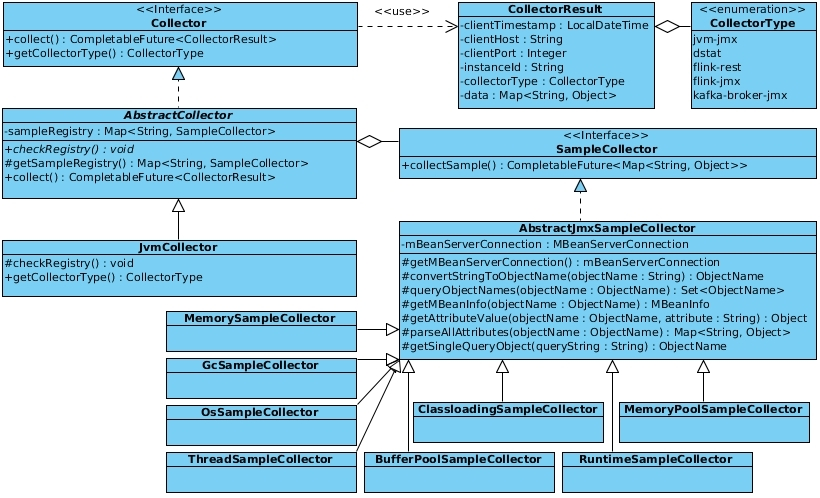
\includegraphics[width=1.0\textwidth]{../uml/class-jvm-collector.jpg}
	\caption{Class diagram 'JvmCollector'}
	\label{class-diagram-jvm-collector}
\end{figure}

This overview describes the collector domain, that is equal to all implementations and consists of following parts:
\begin{enumerate}
    \item \verb|CollectorType|:
    Enumeration, meta information, that distinguishes collectors implementations
    \item \verb|CollectorResult|: Data container, the result of a single invocation of the collect() method from
    the Collector interface. Describes a data event, an immutable fact" at a given time, containing the host and port
    the client is running on, the type of collector and the requested data.
    \item \verb|Collector|: The main interface for implementations, defines the protocol for data collection.
    \item \verb|AbstractCollector|: Abstract class, provides the implementation of the main collect() method.
    \item \verb|SampleCollector|: An interface for all classes that collect samples defined by the group the data
    belongs to.
\end{enumerate}

On the example of \verb|JvmCollector|, the following section explains the basic design principles that is common
to the main collector domain more in detail wheras only relevant implementation details will be discussed in
subsequent implementations, because the process of collecting data is similar in all.

\subsection{JvmCollector}
\label{subsec:impl-jvmcollector}

The implementation of the \verb|Collector| interface for fetching "default" JVM data according to \autoref{tbl:jmxjvmdata}.
This basic set of different management interfaces build the foundation
for the implementation for collecting JVM related data like memory, garbage collector or thread information.

To keep the main implementation as small as possible and following the "Separation Of Concerns" pronciple,
the data was divided into different "sample groups", which resulted in one implementation each for collecting
memory, garbage collector, thread data, et al.

A these \verb|SampleCollector| implementations provide a  \verb|collectSample()| method, that fetches data from a different data group, here
on the example of the class \verb|MemorySampleCollector|.

\begin{lstlisting}[caption={MemorySampleCollector collectSample()}, captionpos=b, label={lst:memory-sample-collect}]
private static final String OBJECT_NAME = "java.lang:type=Memory";

@Override
public CompletableFuture<Map<String, Object>> collectSample() {
    return CompletableFuture.supplyAsync(() -> {
        final Map<String, Object> memoryResultMap = Maps.newLinkedHashMap();
        memoryResultMap.put(SAMPLE_KEY, parseMemory(getMemoryMXBean(OBJECT_NAME)));
        return memoryResultMap;
    });
}

private Map<String, Object> parseMemory(final MemoryMXBean proxy) {
    final Map<String, Object> memoryDataMap = Maps.newLinkedHashMap();
    memoryDataMap.put(MEMORY_OPFC_KEY, proxy.getObjectPendingFinalizationCount());
    return memoryDataMap;
}

private MemoryMXBean getMemoryMXBean(final String objectName) {
    try {
        return ManagementFactory.newPlatformMXBeanProxy(mBeanServerConnection(), objectName, MemoryMXBean.class);
    } catch (IOException ex) {
        throw ex;
    }
}
\end{lstlisting}

As one of the non-functional requirements in \autoref{ch:requirements}, the client implementation may not cause a negative impact
on source systems regarding system resources like cpu or disk usage. To make the code as "non-blocking" as possible,
the implementation is based on the usage of the class \verb|CompletableFuture|. It models an asynchronous computation and provides
a reference to its results that will be available when the computation itself is completed. These computations like the JMX
access in the example above, are potentially time-consuming \cite{Java8}. The \verb|CompletableFuture| allows the caller thread to return immediately
to perform other operations instead of waiting for the result of the computation of JMX memory data, by delegating to a
separate thread performing the operations defined in the \verb|CompletableFuture|.

The code above wraps the computation of JMX memory data, which contains the data access via the MBeanServerConnection,
introduced in \autoref{ch:basic-concepts}, and the preparation of result data in a separate thread performing the operations defined
in the futures method body.

The implementations for the other \verb|SampleCollector|s are almost the same, it only differs in the JMX management bean the data will
be queried from.

Every \verb|Collector| implementation is based on an internal registry of \verb|SampleCollector|s, every implementation must provide its
own registry required for the main  \verb|Collector| process, that delegates to its registered \verb|SampleCollector|s,
aggregates their results and creates the overall result for the \verb|Collector|. To split the collection into individual sample groups has
the advantage, that it makes the implementation very flexible regarding the data to collect. To add further data sources, it
will be enough to provide an implementation of the \verb|SampleCollector| interface and to add an entry to the registry.

\begin{lstlisting}[caption={Sample registry for "JvmCollector"}, captionpos=b, label={lst:jvmsampleregistry}]
private static Map<String, SampleCollector> jvmSampleRegistry(final MBeanServerConnection mBeanServerConnection) {
    final Map<String, SampleCollector> registry = Maps.newHashMap();
    registry.put(MemorySampleCollector.SAMPLE_KEY, new MemorySampleCollector(mBeanServerConnection));
    registry.put(ThreadSampleCollector.SAMPLE_KEY, new ThreadSampleCollector(mBeanServerConnection));
    ...
    return registry;
}

@Override
public CollectorType getCollectorType() {
    return CollectorType.JVM_JMX;
}

@Override
protected void checkRegistry() {
    if (getSampleRegistry().isEmpty()) {
        throw new JmxCollectorException();
    }
}
\end{lstlisting}

The \verb|JvmCollector| implementation only provides the sample registry, the type of collector as well as a simple check if \verb|SampleCollector|s
are registered at all. These methods are defined in the \verb|AbstractCollector| class, discussed in the next section.

\subsection{AbstractCollector}

The abstract base class for all \verb|Collector| implementations that contains the registry of \verb|SampleCollector|s to be used in the main
collection process shown below.

\begin{lstlisting}[caption={"AbstractCollector" sample registry}, captionpos=b, label={lst:abstract-collectorsample-registry}]
private final Map<String, SampleCollector> sampleRegistry;
\end{lstlisting}

The collection process, defined by the \verb|collect()| method in the \verb|Collector| interface is implemented in this abstract class and
therefore the same for all implementations. The only requirement for implementing classes is to provide realizations for the abstract methods in this class.
The following steps are performed:
\begin{lstlisting}[caption={"AbstractCollector" Fetch sample futures}, captionpos=b, label={lst:abstract-collector-step-one}]
final List<CompletableFuture<Map<String, Object>>> sampleResultCPList = getSampleRegistry().values()
    .stream()
    .map(SampleCollector::collectSample)
    .collect(Collectors.toList());
\end{lstlisting}

This demonstrates the Stream features available since Java 8, that enable the processing of collections in a
more functional manner more focussed on the data transformations rather than the data itself. The
implementation creates a Stream of registered \verb|SampleCollector|s, collect the data for each sample and create a list of containing
futures, regarding to to \verb|SampleCollector| interface.

To merge the computations from multiple \verb|SampleCollector|s and extract the the data from \verb|CompletableFuture|s:

\begin{lstlisting}[caption={"AbstractCollector" Merge and extract data }, captionpos=b, label={lst:abstract-collector-step-two}]
final List<Map<String,Object>> sampleResults =
    sampleResultCPList
        .stream()
        .map(CompletableFuture::join)
        .collect(Collectors.toList()))
\end{lstlisting}

\begin{lstlisting}[caption={"AbstractCollector" Create CollectorResult}, captionpos=b, label={lst:abstract-collector-step-three}]
final Map<String, Object> dataMap = Maps.newLinkedHashMap();
sampleResults.forEach(dataMap::putAll);
final CollectorResult collectorResult = new CollectorResult(getCollectorType().name().toLowerCase(),dataMap);
return collectorResult;
\end{lstlisting}

At the end, the \verb|CollectorResult| containing the type and the data will be generated.

The implementations discussed in coming sections are all based on the concept, to divide the collection into separate units and
to create an overall result by aggregating individual sample data. As a result of this approach, the implementations keeps flexible
what makes it easy to add or remove sample data just by providing implementations of the \verb|SampleCollector| interface or removing
an item from the internal registry. In addition, as shown above in the \verb|JvmCollector| class in \autoref{lst:jvmsampleregistry},
the collection of sample data and the
preparation of the \verb|CollectorResult| can be realized with just a few lines of code, which makes the integration of
further data sources quite easy. This will be demonstrated in the coming section.

\subsection{FlinkRestCollector}

This collector implementation fetches data from the HTTP monitoring API that comes with Apache Flink and uses the endpoints
introduced in \autoref{tbl:http-api-flink}.

\begin{figure}[H]
	\centering
	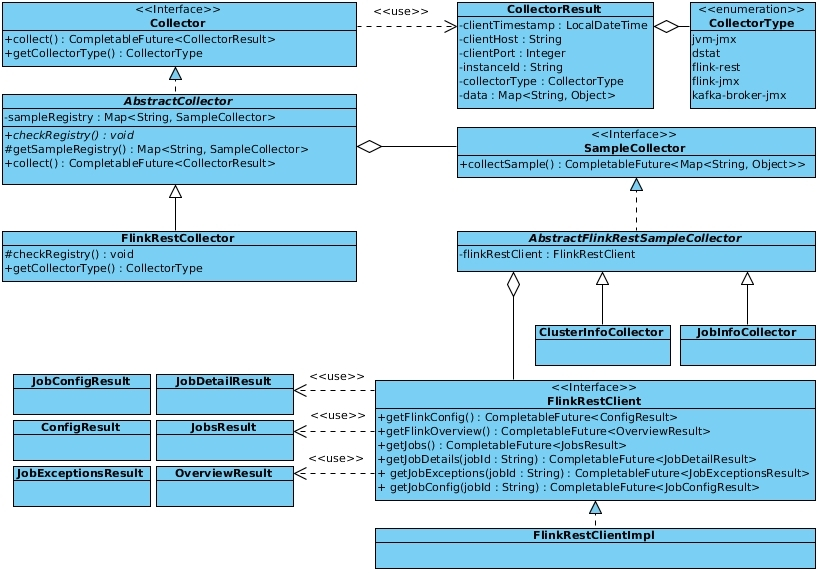
\includegraphics[width=1.0\textwidth]{../uml/class-flink-rest-collector.jpg}
	\caption{Class diagram 'FlinkRestCollector'}
	\label{class-diagram-flink-rest-collector}
\end{figure}

Following the sample approach described above, this \verb|Collector| implementation provides its internal sample registry,
containing the \verb|SampleCollector| implementations based on the data that is desired and shall be collected. Because the monitoring API provides data concerning
general server and cluster information as well as detailed information about jobs and their state, the registry contains
two appropriate \verb|SampleCollector|s:

\begin{lstlisting}[caption={"FlinkRestCollector" Sample registry}, captionpos=b, label={lst:flink-rest-collector-sample-registry}]
private static Map<String, SampleCollector> flinkRestSampleRegistry(final FlinkRestClient flinkRestClient) {
    final Map<String, SampleCollector> registry = Maps.newHashMap();
    registry.put(ClusterInfoCollector.SAMPLE_KEY, new ClusterInfoCollector(flinkRestClient));
    registry.put(JobInfoCollector.SAMPLE_KEY, new JobInfoCollector(flinkRestClient));
    return registry;
}
\end{lstlisting}

The implementation of \verb|SampleCollector| just differs in the way of data access. While the \verb|JvmCollector| uses an \verb|MBeanServerConnection|
to query data using the JMX management interface, \verb|FlinkRestCollector| is based on a REST client internally to request data, which builds
on the \verb|RestTemplate| class, provided by the Spring Framework:

\begin{lstlisting}[caption={"FlinkRestCollector" Rest client}, captionpos=b, label={lst:flink-rest-collector-client}]
final CompletableFuture<OverviewResult> flinkOverviewFuture = restClient().getFlinkOverview();
...
final Map<String, Object> dataMap = Maps.newLinkedHashMap();
dataMap.put(FLINK_JOBS_RUNNING_KEY, flinkOverview.getJobsRunning());
dataMap.put(FLINK_FINISHED_KEY, flinkOverview.getJobsFinished());
dataMap.put(FLINK_CANCELLED_KEY, flinkOverview.getJobsCancelled());
dataMap.put(FLINK_FAILED_KEY, flinkOverview.getJobsFailed());
final Map<String, Object> resultMap = Maps.newLinkedHashMap();
resultMap.put(SAMPLE_KEY, dataMap);
return resultMap;
\end{lstlisting}

By providing this sample data, this \verb|Collector| creates a \verb|CollectorResult| containing the data fetched from Apache Flinks monitoring
API without the need to change the main collector process.

\subsection{DStatCollector}

To collect system related data defined in \autoref{tbl:dstatcategories}, this implementation uses the Dstat system tool,
that provides multiple parameters to specify the data to be displayed. According to the data analysis, following parameters will be used:

\begin{lstlisting}[caption={"DstatCollector" program parameters in }, captionpos=b, label={lst:dstat-parameters}]
private static final String[] DSTAT_COMMAND = {"dstat", "-t",
    "--cpu", "--top-cpu-adv", "--top-cputime", "--top-cputime-avg",
    "--disk", "--disk-tps", "--disk-util",
    "--net", "--socket", "--tcp", "--udp",
    "--io", "--top-io-adv", "--lock", "--fs",
    "--mem", "--top-mem", "--page", "--swap", "--vm",
    "--sys", "--load", "--ipc", "--unix",
    "--proc", "--proc-count", "--top-latency", "--top-latency-avg",
    "--full",
    "--float", "1", "0"};
\end{lstlisting}

According to the given parameters, the \verb|DstatCollector| class is based on the implementations for \verb|CpuSampleCollector|,
\verb|DiskSampleColletor|, etc., which will have to be registrered using a sample registry, as discussed in the sections above.

Starting the Dstat process with the given parameters results in string containing three lines, where only the third line ist required to
to gather data of. To start the external process and to retrieve the resulting output, a \verb|ProcessBuilder| is used, which is part of
the java.lang package.
\begin{lstlisting}[caption={ProcessBuilder in "DstatCollector"}, captionpos=b, label={lst:dstatprocessbuilder}]
final ProcessBuilder processBuilder = new ProcessBuilder(DSTAT_COMMAND);
processBuilder.redirectErrorStream(true);
final Process process = processBuilder.start();
try (BufferedReader processOutputReader =
    new BufferedReader(new InputStreamReader(process.getInputStream()))) {
        final String dstatResult = processOutputReader.lines()
            .map(String::toString)
            .collect(Collectors.joining(System.lineSeparator()));
        final int exitCode = process.waitFor();
}
\end{lstlisting}

All Dstat sample collectors are based on regular expressions, the third line of the result is splitted, and the data of interest
extracted:
\begin{lstlisting}[caption={"CpuSampleCollector", Extract sample data}, captionpos=b, label={lst:cpusamplecollector}]
final Pattern CPU_USAGE_PATTERN = Pattern.compile("" +
    "(\\d+(\\.\\d+)?)(\\s*)" +
    "(\\d+(\\.\\d+)?)(\\s*)" +
    "(\\d+(\\.\\d+)?)(\\s*)" +
    "(\\d+(\\.\\d+)?)(\\s*)" +
    "(\\d+(\\.\\d+)?)(\\s*)" +
    "(\\d+(\\.\\d+)?)")
...
final Matcher matcher = CPU_USAGE_PATTERN.matcher(raw.trim());
final Map<String, Object> cpuUsageMap = Maps.newLinkedHashMap();
if (!matcher.matches()) {
    LOG.warn("Unable to parse 'CpuUsage'");
} else {
    try {
        cpuUsageMap.put(CPU_NAME_KEY, cpuName);
        cpuUsageMap.put(CPU_USAGE_USER_KEY, Float.valueOf(matcher.group(1)));
        cpuUsageMap.put(CPU_USAGE_SYSTEM_KEY, Float.valueOf(matcher.group(4)));
        ...
        } catch (NumberFormatException ex) {
            LOG.warn("Unable to parse 'CpuUsage'");
        }
}
\end{lstlisting}

\subsection{FlinkJmxCollector and KafkaBrokerJmxCollector}

The collection of application data using JMX for Apache Flink and Apache Kafka is working in the
same way as discussed in the previous sections. The implementations both provide \verb|SampleCollector|s for collecting data
from the managed resources which are listed for Apache Kafka in Appendix A by using a \verb|MBeanServerConnection| and querying the resources by their JMX ObjectName,
see \autoref{ch:basic-concepts}. Since Apache Flink is just providing a very basic set
of application data in its current version, containing rudimentary JVM data like cpu load and basic information about current
jobs and their state, this data will be collected nevertheless. It will be assumed to the metric system will be improved in upcoming versions
of Apache Flink. Furthermore the data is redundant, because the implementation of the \verb|JvmCollector| and \verb|FlinkRestCollector| provides a
more detailed set of JVM and job data.

\section{CollectorClient}
\label{sec:impl-collector-client}

After discussing the \verb|Collector| implementations in the previous section, this section introduces the \verb|CollectorClient|,
the core software component representing the entry point for bringing data into the system. This is the component that needs be
installed on Apache Flink and Apache Kafka source systems and has the following responsibilities:

\begin{enumerate}
    \item Register itself on application start with client-discovery
    \item Provide metadata for the \verb|CollectorManager| component available via REST resource
    \item Provide an interface to trigger data collection "on demand" from the \verb|CollectorManager|s web UI
    \item The main collection process, based on registered \verb|collector| implementations
    \item Transport data to the message broker
\end{enumerate}

\begin{figure}[H]
	\centering
	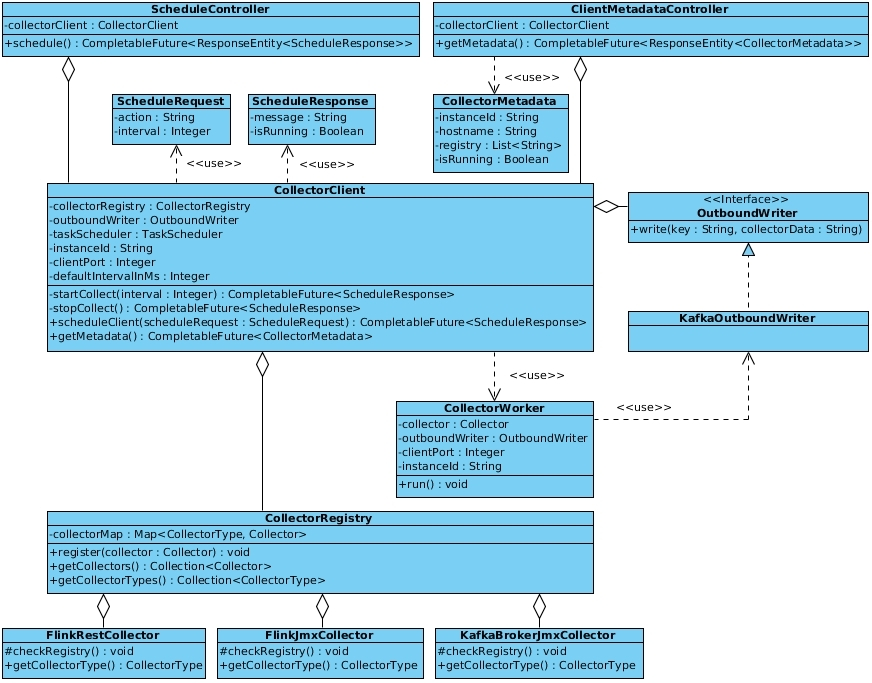
\includegraphics[width=1.0\textwidth]{../uml/class-collector-client.jpg}
	\caption{Class diagram 'CollectorClient'}
	\label{class-diagram-collector-client}
\end{figure}

The \verb|CollectorClient| is a small web service, a self-containing jar-file with an embedded Jetty servlet container realized using
Spring Boot. To register the client with the \textit{Consul Client-Registry}, Spring provides an annotation-based approach to accomplish
this functionality within spring-cloud sub-project, a set of tools for the development of cloud-based applications following common patters
of distributed systems like configuration management, cluster state, service-discovery, etc. .

\begin{lstlisting}[caption={"CollectorClientApp", Client registration}, captionpos=b, label={lst:collector-client-registration}]
@SpringBootApplication
@EnableDiscoveryClient
public class CollectorClientApp {

    public static void main(String[] args) {
        SpringApplication.run(CollectorClientApp.class, args);
    }
}
\end{lstlisting}

The \verb|@EnableDiscoveryClient| annotation seen above requires a Maven dependency to the \verb|spring-cloud-starter-consul-all| artefarct,
which provides and implementation to register the annotated Spring Boot application within the Consul service discovery. Based
on usefull default configurations, this application registers itself the default Consul host \verb|localhost| and port \verb|8500| and is
available to be discovered by the \verb|CollectorManager| component.

The \verb|CollectorClient| provides a Restful web service for fetching metadata for the respective client. This resource is required by
the \verb|CollectorManager| component for displaying detailed client data in the user interface.

\begin{lstlisting}[caption={"ClientMetadataController", Metadata REST endpoint}, captionpos=b, label={lst:metadata-endpoint}]
@Async
@RequestMapping(value="/client/metadata", method = RequestMethod.GET, produces = APPLICATION_JSON_VALUE)
public CompletableFuture<ResponseEntity<CollectorMetadata>> getMetadata() {
    LOG.debug("Entering getMetadata()");
    final CompletableFuture<ResponseEntity<CollectorMetadata>> responseCP = collectorClient.getMetadata()
        .thenApply(metadataMap -> {
            LOG.debug("Fetched client metadata: {}", metadataMap);
            return new ResponseEntity<>(metadataMap, HttpStatus.OK);
        });
        LOG.debug("Immediately return from getMetadata()");
        return responseCP;
    }
\end{lstlisting}

Both code snippets are a good examples for the "minimum of fuss" required to enable small web based services that registers itself
with a service-discovery server. In addition, the last snippet enables a REST resource, localized by the API
path \verb|/client/metadata|, listening for \verb|GET| requests and delivering metadata of the client in JSON format. Furthermore, the capabilities
of asynchronous computations is demonstrated, the \verb|@Async| annotation in combination with the future implementation as the return
value forces the framework to return immediately and not to block the caller thread, see \autoref{subsec:impl-jvmcollector}. Internally,
Spring Boot uses an \verb|ExecutorPool| for the execution of asyncronous computations in a different thread.

In analogy to the metadata enpoint seen above, the client realizes a uniform REST interface that enables the scheduling
of the data collection process. In this case, the servive expects \verb|POST| requests, that contain a \verb|ScheduleRequest| in their
request body provided by the clients that use this service. This body must be JSON formatted and contains the action to
trigger(start/stop data collection) and the time intervall between each collection process, five seconds for example. As result,
a JSON response will be returned, containg a status of the schedule request and the status of the \verb|CollectorClient| (running/stopped).

\begin{lstlisting}[caption={"ScheduleController", REST endpoint}, captionpos=b, label={lst:schedule-endpoint}]
@RequestMapping(value = "/client/schedule", method = RequestMethod.POST, consumes = APPLICATION_JSON_VALUE)
public CompletableFuture<ResponseEntity<ScheduleResponse>> schedule(@RequestBody @Valid final ScheduleRequest request,
    final BindingResult errors) {
LOG.debug("Received schedule request, action={}, interval={}", request.getAction(), request.getInterval());
    if (errors.hasErrors()) {
        throw new CollectorClientException("Invalid schedule request");
    }
    return collectorClient.scheduleClient(request)
        .thenApply(collectorScheduleResponse ->
            new ResponseEntity<>(collectorScheduleResponse, HttpStatus.OK));
}
\end{lstlisting}

Whereas the REST services seen above just take HTTP requests, the \verb|CollectorClient| contains the implementation for
collecting the data based on the concept of a registry of \verb|Collector|s. In contrast to the sample registry explained in the
\verb|Collector| implementations above, the registry holds the \verb|Collector|r implementations, and not any \verb|SampleCollector| which
are part of the \verb|Collector|s. The decoupling of \verb|Collector| implementations from the \verb|CollectorClient| by using a dynamic registry
allows to add further \verb|Collector|s and to remove existing ones without changing the \verb|CollectorClient| implementation.

The scheduling of the client uses Spring's \verb|TaskScheduler| interface that abstracts the scheduling of tasks based on different
kinds of triggers, where a task is an implementation of the \verb|Runnable| interface, defined in the Java core package \verb|java.lang.thread|.
Based on a Stream of registred \verb|Collector| implementations, the client creates instances of the \verb|CollectorWorker| class, that
encapsulates the collection process for execution in a separate thread which will be provided to the task \verb|TaskScheduler|.

\begin{lstlisting}[caption={"CollectorClient", collector registry}, captionpos=b, label={lst:collector-client-registry}]
private List<ScheduledFuture<?>> collectorTaskFutures = null;
...
collectorTaskFutures = collectorRegistry.getCollectors()
    .stream()
    .map(collector -> new CollectorWorker(collector, clientPort, outboundWriter, instanceId))
    .map(collectorWorker -> taskScheduler.scheduleWithFixedDelay(collectorWorker, interval))
    .collect(Collectors.toList());
\end{lstlisting}

The \verb|CollectorWorker| implements \verb|Runnable| interface, hence it must provide an implementation of the parameter-less
\verb|run()|-method. Within its implementation, it fetches the \verb|CompletableFuture| containing collected data, creates a \verb|CollectorResult|
and enriches it with client information, that makes the data set uniquely identifiable.

\begin{lstlisting}[caption={"CollectorWorker", collector registry}, captionpos=b, label={lst:collector-worker}]
private final Collector collector;
private final OutboundWriter outboundWriter;
...
@Override
public void run() {
    LOG.debug("Collector worker starts...");
    collector.collect()
        .thenAccept(collectorResult -> {
            try {
                final CollectorResult result = new CollectorResult(collectorResult.getCollectorType(),
                    collectorResult.getData(), now(), InetAddress.getLocalHost().getHostAddress(),
                                clientPort, instanceId);
                final String jsonData = JsonUtils.toJson(result);
                outboundWriter.write(collector.getCollectorType().name().toLowerCase(), jsonData);
            } catch (UnknownHostException ex) {
                throw new CollectorClientException(ex.getMessage());
            }
    });
    LOG.debug("Collector worker finished");
}
\end{lstlisting}

After the result is created, it will be transfered into its JSON representation and written into a Apache Kafka topic, by using
the \verb|OutboundWriter| interface, whose implementation \verb|KafkaOutboundWriter| uses the class \verb|KafkaTemplate|, provided by the Spring sub-project spring-kafka.

\begin{lstlisting}[caption={"KafkaOutboundWriter", Send data}, captionpos=b, label={lst:outbound-writer}]
private final KafkaTemplate<String, String> kafkaTemplate;
private final String kafkaOutboundTopic;
...
@Override
public void write(final String key, final String jsonData) {
    LOG.debug("Trying to send data to Kafka");
    final ListenableFuture<SendResult<String, String>> sendResultFuture =
        kafkaTemplate.send(kafkaOutboundTopic, key, jsonData);
    sendResultFuture.addCallback(new ListenableFutureCallback<SendResult<String, String>>() {
        @Override
        public void onSuccess(final SendResult<String, String> response) {
                LOG.debug("Successfully send data to Kafka, topic={}, key={}", kafkaOutboundTopic, key);
        }

        @Override
        public void onFailure(final Throwable ex) {
            final OutboundWriterException exception = new OutboundWriterException(format("Error sending data to Kafka: %s", ex.getMessage()));
            LOG.warn(exception.getMessage());
            throw exception;
        }
    });
}
\end{lstlisting}
At this point, the collection process is finished. After the collection interval elapsed, which is configured to be five seconds as
default value, everything will be triggerd again by the \verb|TaskScheduler| described above.

\section{CollectorManager}

The \verb|CollectorManager| is a small web appliction representing the management component in the \textit{"Collector-Platform"}, it
realizes a basic HTML based user interface and provides an overview of all clients registred in the platform as well as a
detailed view of individual clients. In addition, the data collection process can be triggered by using this interface.

\begin{figure}[H]
	\centering
	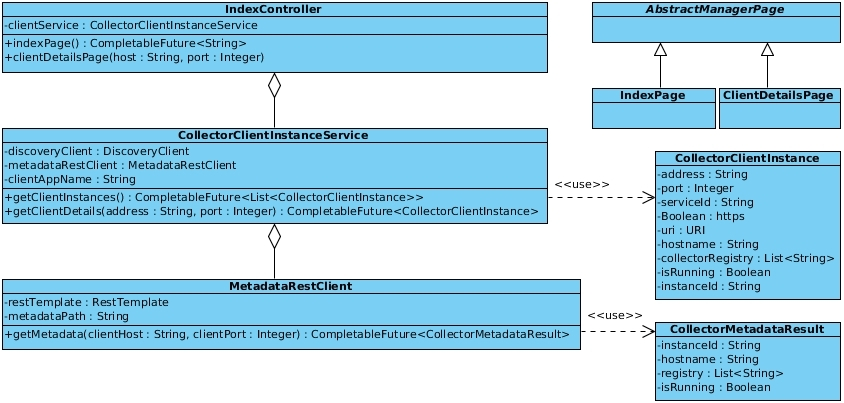
\includegraphics[width=1.0\textwidth]{../uml/class-collector-manager.jpg}
	\caption{Class diagram 'CollectorManager'}
	\label{class-diagram-collector-manager}
\end{figure}

To retrieve the required information of which clients exist and are registered in the system platform, the \verb|CollectorManager|
uses the \verb|DiscoveryClient| implementation provided by spring-cloud.

\begin{lstlisting}[caption={"CollectorClientInstanceService", Get client instances}, captionpos=b, label={lst:client-instance-service}]
private final DiscoveryClient discoveryClient;
private MetadataRestClient metadataRestClient;
...
final List<CollectorClientInstance> clients = discoveryClient.getInstances(clientAppName)
    .stream()
    .map(serviceInstance ->
        CollectorClientInstance.of(serviceInstance.getHost(), serviceInstance.getPort(), serviceInstance.getServiceId(),
        serviceInstance.isSecure(), serviceInstance.getUri())).collect(Collectors.toList());
        LOG.debug("Fetched all client instances: {}", clients);
        return clients;
\end{lstlisting}

The \verb|DiscoveryClient| provides access to the Consul Client-Registry and makes a list of all registered \verb|CollectorClient|s
available that will be displayed in the user interface. In addition, it sends a REST request to the \verb|CollectorClient| itself to enrich
existing Consul data with metadata provided by client as seen in the \verb|CollectorClient| implementation above.

\section{Summary}

The last chapter discussed implementation details for existing data collectors available for Apache Flink and and Apache Kafka.
It introduced the concept of a "sample registry", that divides the main data collection into separate units of work, represented
by implementations of the \verb|SampleCollector| interface. The "main" collectors, means classes that implement the \verb|Collector|
interface, aggregate an overall result based on individual data from multiple \verb|SampleCollector|s.

The \verb|CollectorClient| is based on implementations of the \verb|Collector| interface, which are also organized by an internal registry.
It represents a small REST-based web service that manages the collection process based on registered \verb|Collector|s and provides a REST
interface to enable the collection of data "on-demand".

The \verb|CollectorManager| acts a client for the web services provided by the \verb|CollectorClient|. It uses the REST resources discussed
for listing registered clients, showing detailed client information and starting and stopping the collection process in a basic
HTML-based user interface.

Wheras the \verb|Collector| implementations do not depend on Spring Boot, the framework is used to realize the \verb|CollectorClient| and
\verb|CollectorManager| applications. It enables the development of standalone, self-contained applications with less efford and makes
the integration of 3rd party applications or frameworks, in this example Apache Kafka and Consul, very easy.

The next chapter introduces the local test environment and explains the setup of the prototype application to enable the
evaluation of the software solution according to the requirements defined in \autoref{ch:requirements}. \clearpage
\chapter{Test and Evaluation}
\label{ch:evaluation}
%Aufbau der Messumgebung (1­2 Seiten)
%●
%Server/Betriebssystem etc.
%Datensätze
%Anfragen
%Systeme/Ansätze gegen die Sie sich vergleichen
%Wie messen Sie? Methodik und Maßeinheiten?
%Ist die Messung signifikant?
%Hypothesen/ Was erwarten Sie?
%
%Ergebnisse und Beobachtungen (3 ­4 Seiten)
%●
%Beschreibung  der Ergebnisse
%Diagramme
%Darstellen von Zusammenhängen
%Diskussion und Bewertung (3 ­4 Seiten)
%●
%Wurden Sie überrascht?
%Stimmten Ihre Hypothesen?
%Sind Sie besser, anders als das andere System?
%Wichtigster Erkenntnisgewinn 1
%Wichtigster Erkenntnisgewinn 2
%... .
%Wichtigster Erkenntnisgewinn N
%Anwendbarkeit? Szenario?
%Zusammenfassung (ca. 0,5 Seiten)
%●
%Was haben wir in diesem Kapitel gelernt?
%Wie passt das zur Zielstellung der Arbeit
%Wie passt das zum nächsten Kapitel?
%
%In this section, we will focus on testing and evaluating implemented profiling solution. Testing
%is necessary and extremely important phase in software development lifecycle. For testing
%purposes, we have chosen several approaches:
% manual testing of chosen test scenarios,
% profiling overhead testing with for this purposes designed application,
% profiling overhead and general testing with midPoint
% Automatic testing with unit tests,
%\section{Automated test environment}

The last chapter discussed implementation details for the \textit{"Collector-Platform"} introduced in \autoref{ch:architecture}.
For its realization, Java 8 as programming language head been chosen in combination with the Spring Boot framework which allowed
the rapid implementation of self-containing, distributed applications.

In this section, the focus will be on testing and evaluating the proposed system solution to ensure compliance with the criteria
defined in \autoref{sec:fr} and \autoref{sec:nfr}.

\section{Automated Tests}

A significant approach for testing software products are automated tests that will be executed in the building process.
In Java, unit tests are used for this purpose. The \textit{Collector-Platform} uses Maven as Build-Managemement solution,
that mean the provided test implementations in form of JUnit test classes will be triggered automatically and the sucessfull passing
all existing test cases is a requirement for a successfull building process.

The \textit{"Collector-Platform"}

test
it
coverage



%Prerequisites:
%
%* [java 8](http://www.oracle.com/technetwork/java/javase/downloads/index.html)
%* [maven](https://maven.apache.org/install.html)
%* [docker](https://docs.docker.com/engine/installation/)
%* [docker-compose](https://docs.docker.com/compose/install/
%
%The application was developed and is working with the following software components:
%
%* ubuntu 16.04 LTS
%* oracle java 8
%* maven 3.3.3
%* docker 1.11.2
%* docker-compose 1.7.1

Unit- and Integration tests, IT needs docker infrastructure, usually mocked JMX, REST data,
lack of time, test separation via naming *Test and *IT via Maven Failsafe, check test coverage,
%
%5.4 Automatic Tests
%Another significant approach to testing software products are automatic tests. In java, unit tests
%are used for this purpose. We have implemented automatic tests in our solution using maven
%project management tool and TestNG framework, which provides similar functionality as
%JUnit framework with several new features.
%Scenarios in automatic tests are not that different from scenarios used in automatic
%testing. Main difference is, that in manual tests, living person needed to use applications GUI to
%perform actions defined in test scenarios, while in automatic tests, these test scenarios are
%written as standard java methods with corresponding annotations and no interaction with GUI is
%needed, we simply call specific methods to complete test scenarios (same methods are called in
%manual testing, except they are invoked by user interaction with GUI). For automatic tests, we
%also need to prepare set of test data, for example create necessary profiling objects. We can
%create them programmatically in code of current test code, or prepare them in form of XML and
%parse them during test execution.

\section{Docker environment}

local cluster
Short Docker intro, benefits in microservice environments, describe setup for components (docker-compose.yml),
describe modifications made for Apache Flink and Apache Kafka to enable JMX remote access

\begin{figure}[H]
	\centering
	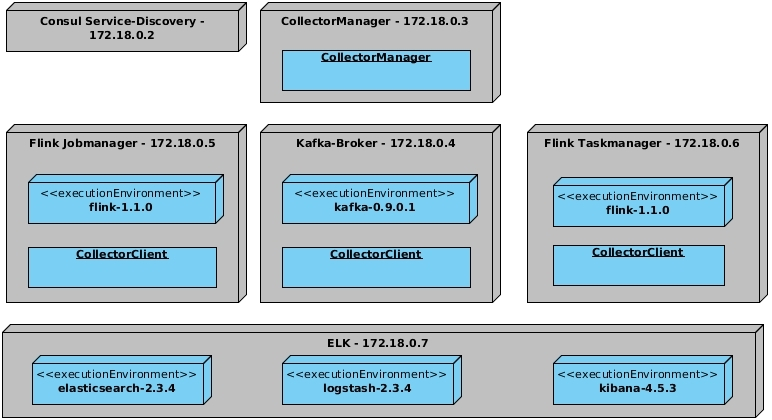
\includegraphics[width=1.0\textwidth]{../uml/deployment-diagram.jpg}
	\caption{Docker Deployment diagram}
	\label{img:deployment-diagram}
\end{figure}

Build images



%\section{Observations}
%
%CollectorDataProcessor: module to analyze the data streams creating derived streams and persist flat
%data -> data transformation, analytics layer
%
%Kibana dashboard, show visualization of CollectorDataProcessor data

\section{Discussion}
%Wurden Sie überrascht? Stimmten Ihre Hypothesen? Sind Sie besser, anders als das andere System?
%Wichtigster Erkenntnisgewinn 1
%Wichtigster Erkenntnisgewinn 2
%Wichtigster Erkenntnisgewinn N
%Anwendbarkeit? Szenario?
\section{Summary}

TODO

%Beschreibung  der Ergebnisse, Diagramme, Darstellen von Zusammenhängen \clearpage
\chapter{Conclusion}
\label{ch:conclusion}

The last chapter \autoref{ch:evaluation} presented the evaluation of the \textit{"Collector-Platform"} based on a multi node cluster
build with the Docker software container engine, that allows to run the required infrastructure components of the platform
on the local developer machine.

This last chapter summarizes the results of the previous chapters and discusses possible optimizations and alternatives to
the chosen approaches of frameworks and technologies.

\section{Summary}

The main goal of the thesis is the design and implementation of a working software system
to ingest and store data that can be collected from Apache Flink and Apache Kafka and
represents the potential data providing component for a the self-learning system, that will be developed within
germans biggest Big Data research project "Berlin Big Data Center".


%Zusammenfassung und Ausblick (5 Seiten)
%●
%●
%●
%Was lesen wir in diesem Kapitel?
%Und warum muss ich das (als Gutachter oder Interessent lesen)?
%Wie verknüpft sich dieser Inhalt mit dem vorhergehendem(n) Kapitel (n)?
%Zusammenfassung
%●
%●
%●
%●
%Was war die Zielstellung?
%Wie war unsere Vorgehensweise?
%Konnten wir das Problem/die Probleme lösen?
%Wichtigste Erkenntnisgewinne?
%Ausblick
%●
%●
%●
%Was würden Sie an dem Thema machen wenn Ihnen jetzt jemand die nächsten drei Jahre
%finanziert?
%Was würde Google / Oracle / IBM machen?
%Sollten wir eigentlich solche Dinge, die Sie in Ihrer Arbeit machen, auch wirklich erforschen
%oder bauen? Wer verliert dadurch, wer gewinnt?


\section{Outlook}

Unit-Test und Refactoring

Maybe Spring alternatives, Lagom, VertX, Play?

Maybe collector as agent, Instrumentation instead of separate service

Alternatives REST, maybe (Web-)Sockets

Possible secururity risk because remote JMX, firewalls and dstat process

More performance with more "system" languages, go? c?

dynamic sample collectors
 \clearpage

%\chapter{Beispiele} \label{c:beispiele}

Im Kapitel Beispiele (siehe \autoref{c:beispiele}) werden die möglichen Funktionen und\index{und} Möglichkeiten dies LaTeX-Dokuments demonstriert.

\section{Quelltext}

Nachfolgend der \autoref{lst:helloworld}.

\begin{lstlisting}[caption={Hello World}, captionpos=b, label={lst:helloworld}]
/**
* The HelloWorldApp class implements an application that
* simply prints "Hello World!" to standard output.
*/
class HelloWorldApp {
	public static void main(String[] args) {
		System.out.println("Hello World!"); // Display the string.
	}
}
\end{lstlisting}

\section{Bild}

\begin{wrapfigure}{R}{0.5\textwidth}
	\centering
	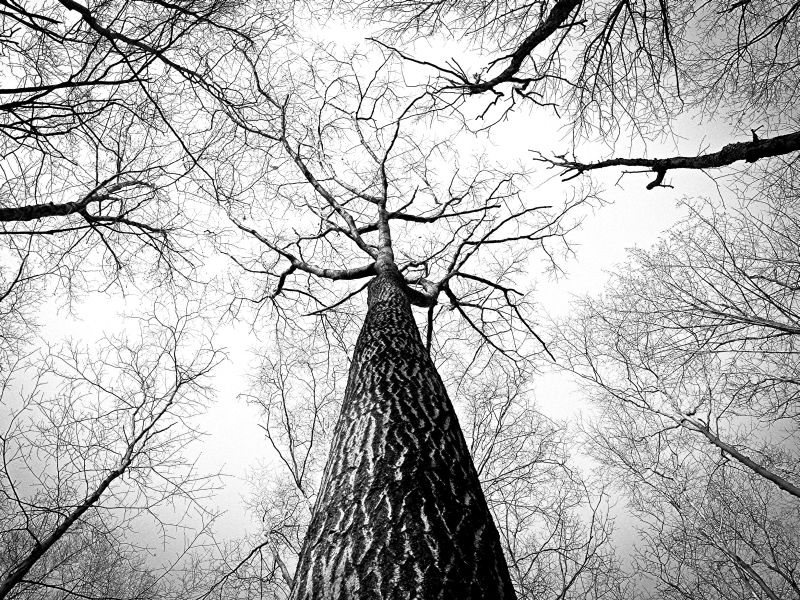
\includegraphics[width=0.5\textwidth]{resources/example}
	\caption{Beispielbild {\cite{PEXELS2015}}}
\end{wrapfigure}

Die rechts zu sehende Grafik demonstriert die Möglichkeiten des Paketes \glqq wrapfig\grqq . Grafiken innerhalb einer \glqq wrapfigure\grqq{} können entweder links oder rechts von Text umlaufen werden.

Die nachfolgende \autoref{img:beispielbild} demonstriert die Darstellung\index{Darstellung} eines \glqq *.jpg\grqq{} Bildes innerhalb des Textes (beim Einfügen kann auf die Endung verzichtet werden, solange der Name einzigartig ist). Zusätzlich enthält dieses einen Untertitel der über das bereits verwendete Label verlinkt werden kann. Der Untertitel\index{Untertitel} erscheint im \gls{abbvz}.

\section{Text Formatierungen und sonstiges}
Dieser Text enthält eine Fußnote\footnote{Fußnoten sind Anmerkungen, die im Druck-Layout aus dem Fließtext ausgelagert werden, um den Text flüssig lesbar zu gestalten.}.

\subsection{Listen}
Listen könne sowohl mit Bullet points als auch mit Zahlen erstellt werden
\begin{itemize}
	\item Eine Liste mit Bullet points
	\item Ein weiteres Element
\end{itemize}

\begin{enumerate}
	\item Eine Liste mit Zahlen
	\item Ein weiteres Element
\end{enumerate}

\subsection{Text Hervorhebungen}
\begin{quote}
	The problem with internet quotes is that you can't always depend on their accuracy \par\raggedleft--- \textup{Abraham Lincoln, 1864}
\end{quote}

"Inspirierende Zitate können mit epigraph eingefügt werden
\epigraph{The problem with internet quotes is that you can't always depend on their accuracy}{Abraham Lincoln, 1864}

Seitenumbrüche können nur direkt nach Text geschrieben werden, sonst lässt sich das Latex nicht mehr compilieren.
\\

\begin{figure}[H]
	\centering
	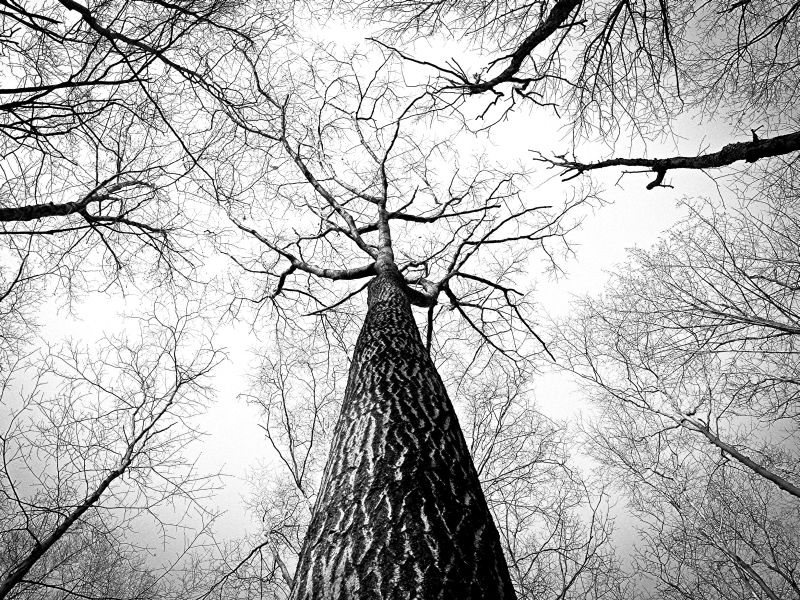
\includegraphics[width=0.7\textwidth]{resources/example}
	\caption{Beispielbild {\cite{PEXELS2015}}}
	\label{img:beispielbild}
\end{figure}

\section{Tabelle}

Nachfolgend \autoref{tbl:DigitalesZertifikat}.

\begin{table}[H]
	\begin{center}
		\renewcommand{\arraystretch}{1.3}
		\begin{tabular}{|l|}
			\hline
			\textbf{Inhaber:}\\
			Alice \\ \hline
			\textbf{Peer (Ersteller):}\\
			Bob \\ \hline
			\textbf{Öffentlicher Schlüssel des Inhabers:}\\
			F2 D2 0E ED FA 4E 9E 0A F2 DD 23 8A 32 44 F3 E9 \\ \hline
			\textbf{Gültigkeit:}\\
			2015-07-01 – 2016-06-30 \\ \hline
		\end{tabular}
	\end{center}
	\caption{Digitales Zertifikat}
	\label{tbl:DigitalesZertifikat}
\end{table}

\section{Long-Table}

Die \glqq Long-Table\grqq kann über definierte Header und Footer über Seitenumbrüche hinweg angezeigt werden.

\begin{longtable}{|l|l|l|l|}
	\hline
	\multicolumn{1}{|c}{\textbf{Version}} & \multicolumn{1}{|c}{\textbf{Codename}} &
	\multicolumn{1}{|c}{\textbf{API}} &
	\multicolumn{1}{|c|}{\textbf{Verteilung}} \\ \hline
	\endfirsthead
	
	\multicolumn{4}{c}{Fortsetzung - Verteilung der Androidversionen (Stand 01.02.2016)}\\ \hline
	\multicolumn{1}{|c}{\textbf{Version}} & \multicolumn{1}{|c}{\textbf{Codename}} &
	\multicolumn{1}{|c}{\textbf{API}} &
	\multicolumn{1}{|c|}{\textbf{Verteilung}} \\ \hline 
	\endhead
	
	\multicolumn{4}{c}{Fortsetzung auf nachfolgender Seite}
	\endfoot
	
	\caption{Verteilung der Androidversionen (Stand: 01.02.2016)}
	\label{tab:androidverteilung}
	\endlastfoot
	
	2.2 & Froyo & 8 & 0.1\%\\ \hline
	2.3.3 - 2.3.7 & Gingerbread & 10 & 2.7\%\\ \hline
	4.0.3 - 4.0.4 & Ice Cream Sandwich & 15 & 2.5\%\\ \hline
	4.1.x & Jelly Bean & 16 & 8.8\%\\ \cline{1-1} \cline{3-4}
	4.2.x &  & 17 & 11.7\%\\ \cline{1-1} \cline{3-4}
	4.3 &  & 18 & 3.4\%\\ \hline
	4.4 & KitKat & 19 & 35.5\%\\ \hline
	5.0 & Lollipop & 21 & 17.0\%\\ \cline{1-1} \cline{3-4}
	5.1 &  & 22 & 17.1\%\\ \hline
	6.0 & Marshmallow & 23 & 1.2\%\\ \hline
\end{longtable}

\section{Literaturverweis}

Weil für die alte\index{alte} und die neue Rechtschreibung verschiedene Trennregeln\index{Trennregeln} gelten, sind Deutsch mit alter Rechtschreibung und Deutsch mit neuer Rechtschreibung zwei verschiedene Sprachen (\cite{Knappen2009}, S. 192).

\section{Onlineverweise}

Siehe Google.de \cite{Google2015}.

\section{Glossar}
Der Glossar enthält die Beschreibung verwendeter Begriffe für das bessere Verständnis gegenüber dem Leser. Beispiele sind: \gls{berlin}, \gls{outsourcing}, \gls{asp}, \gls{policy} und \gls{pcie}.

\section{Abkürzungsverzeichnis}
Das Abkürzungsverzeichnis listet alle verwendeten Abkürzungen auf. Einige Beispiele sind \gls{sas}, \gls{cd}, \gls{lan} und \gls{iso}. Die erneute Verwendung zeigt nur noch die Abkürzung: \gls{sas}, \gls{cd}, \gls{lan} und\index{und} \gls{iso}. \clearpage

\pagenumbering{Alph}
\listoffigures \clearpage
\listoftables \clearpage
\lstlistoflistings \clearpage\textbf{}

\printindex \clearpage

%\printglossary[title={Glossar}] \clearpage
%\printglossary[style=dottedlocations,type=\acronymtype,title={List of abbreviations}] \clearpage

\printbibliography[heading=bibintoc, notkeyword={image}]\clearpage
%\printbibliography [heading=bibintoc, keyword={book}, title={Bibliography}]\clearpage
%\printbibliography[heading=bibintoc, keyword={article}, title={Articles}]\clearpage
%\printbibliography[heading=bibintoc, keyword={online}, title={Online resources}]\clearpage
\printbibliography[heading=bibintoc, keyword={image}, title={Image resources}]\clearpage

% Anhang
\appendix

\chapter{}
\addcontentsline{toc}{chapter}{Appendix A}

\section{Collectors JSON results}
\subsection{JvmCollector}
\subsection{DstatCollector}
\label{subsec:dstat-result}
\subsection{FlinkRestCollector}
\subsection{FlinkJmxCollector}
\subsection{KafkaBrokerJmxCollector}

\section{Apache Flink 1.1.0 API JSON responses}
\verb|GET /jobs|
%\begin{lstlisting}[caption={DStatCollector JSON payload}, captionpos=b, label={lst:dstat-payload}]
%{
%  "jobs-running": [],
%  "jobs-finished": [
%    "df399b48d225cda1a5c0a36ed9519b62",
%    "2efc5e7c9a9f274efbb420a01e6b00cc"
%  ],
%  "jobs-cancelled": [],
%  "jobs-failed": []
%}
%\end{lstlisting}

\section{Apache Kafka 0.9.0.1 MBeans}
\begin{table}[H]
    \begin{tabular}{l}
        \textbf{JMX ObjectName} \\
        kafka.controller:type=ControllerStats,name=LeaderElectionRateAndTimeMs \\
        kafka.controller:type=ControllerStats,name=UncleanLeaderElectionsPerSec \\
        kafka.controller:type=KafkaController,name=ActiveControllerCount \\
        kafka.controller:type=KafkaController,name=OfflinePartitionsCount \\
        kafka.controller:type=KafkaController,name=PreferredReplicaImbalanceCount \\
        kafka.network:type=Processor,name=IdlePercent,networkProcessor=* \\
        kafka.server:type=socket-server-metrics,networkProcessor=* \\
        kafka.server:type=controller-channel-metrics,broker-id=* \\
        kafka.server:type=ReplicaManager,name=IsrExpandsPerSec \\
        kafka.server:type=ReplicaManager,name=IsrShrinksPerSec \\
        kafka.server:type=ReplicaManager,name=LeaderCount \\
        kafka.server:type=ReplicaManager,name=PartitionCount \\
        kafka.server:type=ReplicaManager,name=UnderReplicatedPartitions \\
        kafka.server:type=KafkaRequestHandlerPool,name=RequestHandlerAvgIdlePercent \\
        kafka.server:type=BrokerTopicMetrics,name=TotalProduceRequestsPerSec \\
        kafka.server:type=BrokerTopicMetrics,name=TotalProduceRequestsPerSec,topic=* \\
        kafka.server:type=BrokerTopicMetrics,name=TotalFetchRequestsPerSec \\
        kafka.server:type=BrokerTopicMetrics,name=TotalFetchRequestsPerSec,topic=* \\
        kafka.server:type=BrokerTopicMetrics,name=BytesInPerSec \\
        kafka.server:type=BrokerTopicMetrics,name=BytesInPerSec,topic=* \\
        kafka.server:type=BrokerTopicMetrics,name=BytesOutPerSec \\
        kafka.server:type=BrokerTopicMetrics,name=BytesOutPerSec,topic=* \\
        kafka.server:type=BrokerTopicMetrics,name=BytesRejectedPerSec \\
        kafka.server:type=BrokerTopicMetrics,name=BytesRejectedPerSec,topic=* \\
        kafka.server:type=BrokerTopicMetrics,name=FailedFetchRequestsPerSec \\
        kafka.server:type=BrokerTopicMetrics,name=FailedFetchRequestsPerSec,topic=* \\
        kafka.server:type=BrokerTopicMetrics,name=FailedProduceRequestsPerSec \\
        kafka.server:type=BrokerTopicMetrics,name=FailedProduceRequestsPerSec,topic=* \\
        kafka.server:type=BrokerTopicMetrics,name=MessagesInPerSec \\
        kafka.server:type=BrokerTopicMetrics,name=MessagesInPerSec,topic=* \\
        kafka.coordinator:type=GroupMetadataManager,name=NumGroups \\
        kafka.coordinator:type=GroupMetadataManager,name=NumOffsets \\
    \end{tabular}
    \caption{Collected Kafka MBeans}
    \label{tbl:kafka-controller}
\end{table}

\section{Docker Configuration}
\label{app:docker-config}

\begin{lstlisting}[caption={"Collector-Platform" cluster configuration}, captionpos=b, label={lst:docker-config-all}]
version: '2'
services:

  consul:
    image: "progrium/consul:latest"
    container_name: "consul"
    hostname: "consul"
    ports:
      - "8400:8400"
      - "8500:8500"
      - "8600:53"
    command: "-server -bootstrap-expect 1 -ui-dir /ui"

  zookeeper:
    container_name: zookeeper
    image: wurstmeister/zookeeper
    ports:
      - "2181:2181"

  kafka:
    container_name: kafka
    image: wurstmeister/kafka
    ports:
      - "9092:9092"
      - "9997:9999"   # jmx
      - "9097:9091"   # collector-client
    environment:
      KAFKA_ZOOKEEPER_CONNECT: zookeeper:2181
      KAFKA_ADVERTISED_HOST_NAME: 192.168.2.100
      KAFKA_CREATE_TOPICS: "collector-outbound-topic:1:1,flink-outbound-topic:1:1"
      JMX_PORT: 9999
      SPRING_PROFILES_ACTIVE: kafka-broker-jmx
      SPRING_CLOUD_CONSUL_HOST: consul
      SPRING_CLOUD_CONSUL_PORT: 8500
      CLIENT_PORT: 9091
      KAFKA_BROKER_ADDRESS: kafka:9092
    volumes:
      - /var/run/docker.sock:/var/run/docker.sock
    depends_on:
      - zookeeper
      - consul

  flink-jobmanager:
    image: flink
    container_name: flink-jobmanager
    ports:
      - "8081:8081"   # webui
      - "9999:9999"   # jmx
      - "9099:9091"   # collector-client
    command: jobmanager
    volumes:
      - /usr/local/flink/conf
    depends_on:
      - consul
      - kafka
      - elk
    environment:
      SPRING_PROFILES_ACTIVE: dstat,jvm-jmx,flink-jmx,flink-rest
      SPRING_CLOUD_CONSUL_HOST: consul
      SPRING_CLOUD_CONSUL_PORT: 8500
      CLIENT_PORT: 9091
      KAFKA_BROKER_ADDRESS: kafka:9092

  flink-taskmanager:
    image: flink
    container_name: flink-taskmanager
    ports:
      - "9998:9999"   # jmx
      - "9098:9091"   # collector-client
    command: taskmanager
    volumes_from:
      - flink-jobmanager
    depends_on:
      - flink-jobmanager
      - consul
      - kafka
      - elk
    environment:
      SPRING_PROFILES_ACTIVE: flink-rest #,jvm-jmx
      SPRING_CLOUD_CONSUL_HOST: consul
      SPRING_CLOUD_CONSUL_PORT: 8500
      CLIENT_PORT: 9091
      KAFKA_BROKER_ADDRESS: kafka:9092
      FLINK_REST_HOST: flink-jobmanager
      FLINK_REST_PORT: 8081

  elk:
    container_name: elk
    image: sebp/elk
    ports:
      - "5601:5601"
      - "9200:9200"
      - "5044:5044"
      - "5000:5000"
    depends_on:
      - zookeeper
      - kafka

  collector-manager:
    container_name: collector-manager
    image: io.thesis/collector-manager
    ports:
      - "9090:9090"
    depends_on:
      - consul
    environment:
      SERVER_PORT: 9090
      SPRING_CLOUD_CONSUL_HOST: consul
      SPRING_CLOUD_CONSUL_PORT: 8500
\end{lstlisting}

%\section{Diagrams}
%\subsection{Use Case diagram}
%
%\begin{figure}[H]
%	\centering
%	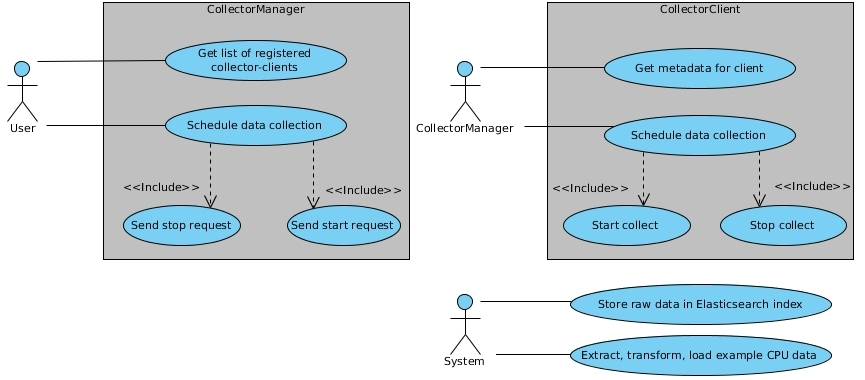
\includegraphics[width=1.0\textwidth]{../uml/usecase-collector-process.jpg}
%	\caption{Use Case Diagramm}
%	\label{use-case-diagram}
%\end{figure}

%\begin{figure}[H]
%	\centering
%	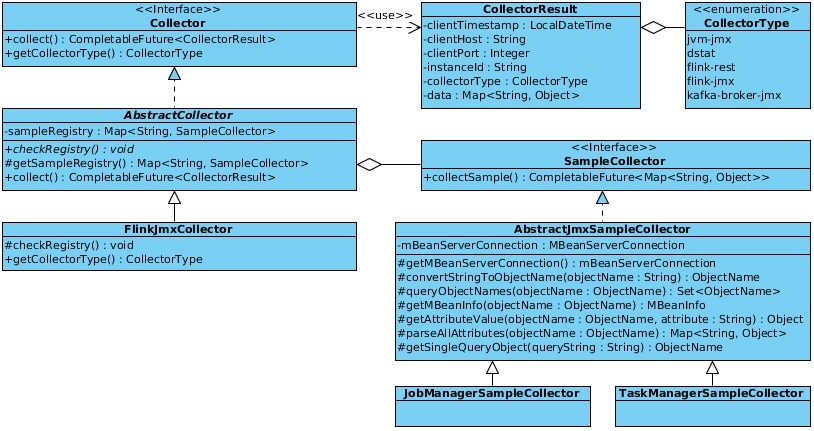
\includegraphics[width=1.0\textwidth]{../uml/class-flink-jmx-collector.jpg}
%	\caption{Class diagram 'FlinkJmxCollector'}
%	\label{class-diagram-flink-jmx-collector}
%\end{figure}
%\begin{figure}[H]
%	\centering
%	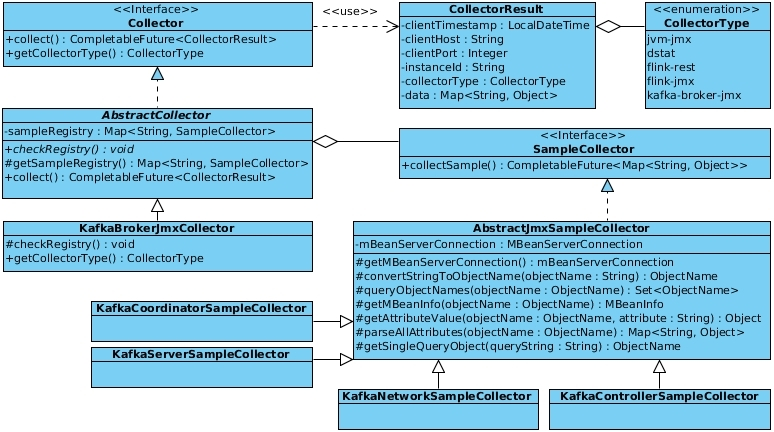
\includegraphics[width=1.0\textwidth]{../uml/class-kafka-broker-jmx-collector.jpg}
%	\caption{Class diagram 'KafkaBrokerJmxCollector'}
%	\label{class-diagram-kafka-broker-jmx-collector}
%\end{figure}

%\subsection{Deployment diagram}






%\begin{lstlisting}[language=json, caption={DStatCollector JSON payload}, captionpos=b, label={lst:dstat-payload}]
%{
%    "clientTimestamp": "2016-08-12T20:59:30.608",
%    "clientHost": "127.0.1.1",
%    "clientPort": 9091,
%    "instanceId": "collector-client:25ba074a0d81dd5c8e2c7b4c73152dd2",
%    "collectorType": "dstat",
%    "data": {
%        "disk": {
%            "read": 112.0,
%            "write": 436.0,
%            "utilization": 6.49,
%            "transactions": {
%                "read": 5.72,
%                "write": 8.9
%            }
%        },
%        "process": {
%            "runnable": 0.0,
%            "uninterruptible": 0.0,
%            "new": 1.4,
%            "count": 271,
%            "latency-highest-total": {
%                "name": "compiz",
%                "value": 8475.0
%            },
%            "latency-highest-avg": {
%                "name": "cat",
%                "value": 101.0
%            }
%        },
%        "memory": {
%            "usage": {
%                "used": 5548032.0,
%                "buffer": 217088.0,
%                "cache": 1626112.0,
%                "free": 695296.0
%            },
%            "process-most-expensive": {
%                "name": "java",
%                "value": 1510400.0
%            },
%            "paging": {
%                "in": 1.22265625,
%                "out": 10.8
%            },
%            "swap": {
%                "used": 312320.0,
%                "free": 7987200.0
%            },
%            "vm": {
%                "hardPageFaults": 0.5,
%                "softPageFaults": 990.0,
%                "allocated": 1476.0,
%                "free": 1500.0
%            }
%        },
%        "system": {
%            "load-avg": {
%                "1m": 1.16,
%                "5m": 1.28,
%                "15m": 1.17
%            },
%            "interrupts": 1225.0,
%            "contextSwitches": 3178.0,
%            "ipc": {
%                "messageQueue": 0.0,
%                "semaphores": 0.0,
%                "sharedMemory": 29.0
%            },
%            "unix-sockets": {
%                "datagram": 38,
%                "stream": 799,
%                "listen": 38,
%                "active": 761
%            }
%        },
%        "io": {
%            "read": 5.72,
%            "write": 8.9,
%            "process-most-expensive": {
%                "name": "upstart",
%                "pid": 3210,
%                "read": 502.0,{
%                "write": 210.0,
%                "cpuPercentage": 0.0
%            },
%            "filelocks": {
%                "posix": 33.0,
%                "flock": 4.0,
%                "read": 13.0,
%                "write": 25.0
%            },
%            "filesystem": {
%                "openFiles": 13344,
%                "inodes": 48582.0
%            }
%        },
%        "cpu": {
%            "usage": [
%                {
%                    "name": "cpu0",
%                    "user": 17.0,
%                    "system": 3.3,
%                    "idle": 77.0,
%                    "wait": 2.6,
%                    "hwInterrupt": 0.0,
%                    "swInterrupt": 0.0
%                },
%                {
%                    "name": "cpu1",
%                    "user": 17.0,
%                    "system": 3.4,
%                    "idle": 77.0,
%                    "wait": 2.7,
%                    "hwInterrupt": 0.0,
%                    "swInterrupt": 0.4
%                }
%            ],
%            "process-most-expensive": {
%                "name": "java",
%                "pid": 32528,
%                "cpuPercentage": 5.8,
%                "read": 102.0,
%                "write": 272.0
%            },
%            "process-cpu-time-highest-total": {
%                "name": "Xorg",
%                "time": 40.1
%            },
%            "process-cpu-time-highest-avg": {
%                "name": "docker-compos",
%                "time": 225.0
%            }
%        },
%        "net": {
%            "traffic": [
%                {
%                    "name": "docker0",
%                    "send": 0.0,
%                    "received": 0.0
%                },
%                {
%                    "name": "wlp2s0",
%                    "send": 0.0,
%                    "received": 0.0
%                }
%            ],
%            "sockets": {
%                "total": 1.0,
%                "tcp": 19.0,
%                "udp": 8.0,
%                "raw": 0.0,
%                "ipFragments": 0.0
%            },
%            "tcp-sockets": {
%                "listen": 20.0,
%                "established": 43.0,
%                "syn": 0.0,
%                "timeWait": 5.0,
%                "close": 0.0
%            },
%            "udp": {
%                "listen": 17.0,
%                "active": 0.0
%            }
%        }
%    }
%}
%\end{lstlisting}

% Eigenständigkeitserklärung
\addchap{Eigenständigkeitserklärung}

Hiermit versichere ich, dass ich die vorliegende Masterarbeit selbstständig und nur unter
Verwendung der angegebenen Quellen und Hilfsmittel verfasst habe. Die Arbeit wurde bisher
in gleicher oder ähnlicher Form keiner anderen Prüfungsbehörde vorgelegt.

\vskip 1cm

Stadt, den xx.xx.xxxx

\vskip 1.5cm

Max Mustermann

\end{document}